% !TeX root = main.tex
\chapter{Background}\label{chp:background}

%Study on TV sport \citep{Perry2009} and \citep{Engstroem2010}

%Review on video interaction tools \citep{Schoeffmann2015}

%Research on navigation of recorded speech for navigating meetings \citep{Bouamrane2007}: speaker segmentation, speech
%skimming, automated speech recognition, word spotting, topic segmentation, spoken language summarisation.

%Review on smart meeting systems \citep{Yu2010}

%\citet{Loviscach2011a} includes low-level features (Comparisonics) and high-level features (keywords from ASR)

%\citet{Tucker2005} provides an overview of multimodal meeting data browsers.

%Audio mixing designs based on data visualization first principles \citep{Dewey2016,Dewey2016a}

In this chapter, we start with a brief overview of radio production and the current tools that producers use to edit
radio programmes.  We show how semantic audio analysis can be used to extract information about the audio content that
describes the sound in human-readable terms.  We then consider previous user interfaces that have used this semantic
data to improve the navigation and editing of audio through visualization, transcripts, and audio playback.  We finish
by considering the research strategy we will use to answer our research questions.

%Stolen: In this chapter, we can find a review of a variety of systems and technologies that are related to the
%approach we have chosen for our search interface. It is organized in sections according to different research fields
%that play an important role on our proposed system.

%TODO
%- interested in reviewing technology that aids navigation and editing of audio
%- Radio is based only on sound, so we will exclude navigation of content through video thumbnails
%- Production of original content uses specific files, so we will exclude navigation of collections and archives

%TODO
% a variety of methods are used through this thesis to evaluate technical interventions, these will be introduced in
% each chapter

%====================================================================================================================
\section{Radio production}\label{sec:background-radio}

%Radio production is ``using sound elements to create an effect or deliver a message'' \citep[p. 12]{Hausman2012}.
%A radio producer is ``anyone who manipulates sound to create an effect or deliver a message'' \citep[p. 19]{Hausman2012}
%Production is ``a method of combining various sources of sound into a product that accomplishes something specific'' \citep[p.~20]{Hausman2012}

% WHAT IS RADIO PRODUCTION?
The focus of this thesis is on the production of audio content for radio broadcast.  Radio production is both a
creative and technical endeavour. The aim of radio production is to ``manipulate sound to create an effect or deliver a
message'', which is achieved by combining various sources of sound into a programme \citep[pp. 12, 20]{Hausman2012}.
Producing radio requires the combination of complex audio technology with artistic taste and judgement
\citep{Barbour2004}.  In this section, we shall start by giving an overview of radio production activities at the BBC,
then describe how the audio content is put together using audio editing.


\subsection{BBC Radio}

% Political structure
% - radio stations, listeners
% - amount spent on production
% - indies, compare to TV

Ten UK-wide radio networks and two national radio services each in Scotland, Wales and Northern Ireland, 40 local radio
stations in England and the Channel Islands. \citep{BBC2017a}

Radio is relatively cheap to produce.
The national BBC radio stations cost between 0.5p and 5.7p per listener hour to produce, which is much lower than
the national television channels, which cost between 3p and 20.9p to produce \citep[pp. 25, 27]{BBC2017a}.

World Service Radio has 154M listeners per week \cite[p.~32]{BBC2017a}.


9 national stations with 34m listeners, 40 local stations with 8m listeners, one global station in 29 languages with
269m listeners

The BBC spent \textsterling471M on radio production in 2016/17 \citep[p. 111]{Ofcom2017}.

%Most radio is broadcast live, where the audience is listening to the radio as it is
%created. However, 


% Production environment
% - OBH since 1932
% - locations, London and Manchester

%Audio production in office environments \citep{Brixen2003}

\subsection{Audio editing}

% benefits of pre-production
The focus of this thesis is on the production of radio programmes that are fully or partly pre-recorded.  Recording
sound ahead of broadcast brings with it a number of benefits \citep[p. 133]{Hausman2012}.  Programmes can be much more
complex, as many more sound elements can be brought together than would be possible in a live scenario.  The producer
is able to record re-takes of the same material until they are satisfied, which allows them greater freedom to
experiment and fix any mistakes that occured.  This paves the way for different types of programmes, such as drama and
documentaries and, in turn, can lead to better quality content.  Pre-recording has a number of practical benefits too.
The time of production is not constrained by the broadcast schedule, so recording can take place whenever is
convenient, and content for multiple programmes can also be recorded in one session, rather than having to come back
each time.

% WHAT IS EDITING?
Pre-recorded audio is produced through editing. \textit{Audio editing} is the process of selecting, re-arranging,
correcting and assembling audio content into a finished product \citep[p. 112]{Hausman2012}.  According to
\citet[p.~44]{McLeish2015} and \citet[p.~116]{Hausman2012}, the three primary reasons for editing are to:

{\singlespacing
\begin{enumerate}
  \item Re-arrange recorded material into a more logical sequence.
  \item Remove uninteresting, unwanted, repetitive or technically unacceptable sound.
  \item Reduce the running time.
\end{enumerate}
}

Although the activities that make up editing are of a practical nature, audio editing is a creative process.
\citet[p.~116]{Hausman2012} states that editing is ``somewhat like an art form'', and \citet[p.~44]{McLeish2015}
suggests that editing can used as a ``creative effect to produce juxtapositions of speech, music, sound and silence''.


\subsection{Digital audio workstations}\label{sec:background-daw}

% what is digital audio?
For more than fifty years, audio was recorded on magnetic tape. Combining sound sources required the use of a large
mixing console which was used to control the sound with faders, knobs and buttons that had to be triggered at the right
time. Editing was performed by cutting the magnetic tape with a razor blade and sticking it back together again
\citep{Barbour2004}.

The development of fast processors and high quality audio interfaces has since allowed audio to
be stored and manipulated digitally. Digital audio is recorded through a process of \textit{sampling}, where an analog
audio signal is converted into a numerical representation.  This digital audio representation can then be read and
manipulated using computer software.
%The amplitude of the signal is measured about 48,000 times a second and saved onto a computer file using binary
%numbers.

% how is digital audio editing peformed?
The primary tool for editing digital audio is the \textit{digital audio workstation}, or \textit{DAW}. A DAW is
software that provides recording, mixing and editing capabilities for digital audio.  DAWs were first introduced in the
1980s \citep{Ingebretsen1982}, and have since evolved into powerful tools that are available to anybody with a
computer. Examples of popular commercial DAWs include Pro Tools by Avid, Logic Pro by Apple and Cubase by Steinberg
\citep{AskAudio2015,ProducerSpot2015}.

% Advantages of DAW:
% - automatic functions (e.g. crossfades that make edits undetectable)
% - non-destructive
% - no loss in sound quality
% - 100\% accuracy
% - fine control over timing
DAWs provide a feature-rich toolset for manipulating audio signals.  They can be used to navigate and edit audio with
very fine control over timing, even down to individual samples. Automation means that changes made to the audio are
remembered and repeated each time the audio is played. Automatic cross-fading between clips can be used to
create inaudible edits.

% how has digital audio changed radio?
% - doesn't require use of a studio
% - programme can be produced by one person
The introduction of DAWs has transformed radio broadcasting by allowing fast random access, high storage densities,
improved portability, and greater cost-effectiveness than analog systems \citep{Pizzi1989}.  The powerful features of a
DAW can replace most of the activities that would traditionally have to be performed using a radio studio.  The
accessibility of digital audio production has allowed audio editing to be performed by producers without requiring
specialist knowledge of sound engineering \citep{Peus2011}. This has caused a reduction in the number of people
required to produce radio programmes \citep{Dunaway2000}.  The ease of digital audio production can also create a
``high level of personal job satisfaction'' \citep[p.~44]{McLeish2015}.

%Digital technology has also changed music recording by allowing people to record at home, and impacted the music
%business \citep{Pras2013}

% destructive vs non-destructive
As the audio is being stored and manipulated digitally, DAWs can be used to edit audio without any loss in sound
quality. However, when the edited audio is saved, there are two approaches that can be taken -- destructive and
non-destructive. \textit{Destructive editing} occurs when a change is made that alters the structure of the sound file.
This means that the edits cannot easily be undone. \textit{Non-destructive editing} occurs when the original audio
components are retained and can be re-used to make a change to the edit. DAWs can perform non-destructive editing by
saving an \textit{edit decision list}, or \textit{EDL}, which records the positions of the edits, but does change any
audio files. With EDLs, audio edits can be moved or undone retrospectively. Only when the final edits are ready does
the audio get destructively ``rendered'' or ``bounced'' to a file.

\subsection{Visual representation}

%``In computer-assisted editing, the information is stored digitally and manipulated through visual representation on a
%computer screen''
Digital audio editing is performed using a visual representation on a computer screen \citep[p. 201]{Hausman2012}.
\citet{Barbour2004} found through observation and interviews with radio producers that ``visualization of audio on a
screen has become the dominant focus in a radio production studio'', and that visual representations are used to
assemble, modify and balance the audio for radio programmes.

% pros and cons of visual representation
Using visual means to interact with audio has a number of benefits. It allows users to manipulate the audio using a
mouse and screen, which are commonly used in computing.  Mapping audio to an image allows the temporal information of
the sound to be displayed spatially, which means it can be searched and skimmed quickly and randomly.  However,
visualizing audio is difficult, and there are limitations to what audio visualizations can tell us about the audio.

As \citet{Bouamrane2007} points out, ``visually representing audio in a meaningful manner is a particularly difficult
task as there is no obvious or intuitive way of doing so''.  Currently visual representations cannot fully represent
the sound, so producers must listen to comprehend the audio.  \citet[p. 45]{McLeish2015} argue that ``while it is
tempting to edit visually using the waveform on the screen, it is essential to listen carefully to the sound, [such as
to] distinguish between an end-of-sentence breath and a mid-sentence breath''.  Visual representations may also serve
as a distraction to the producer.  \citet{Barbour2004} found that to help them concentrate on listening, radio
producers disengaged their visual senses by shutting or de-focusing their eyes, or looking away.

Although we could not find any studies that surveyed the use of visualizations in DAWs, we looked at the five most
popular DAWs \citep{AskAudio2015} and found that all of them visualized the audio using a ``waveform''.

%In this
%section, we will introduce the audio waveform, discuss its pros and cons, and compare it to an alternative
%visualization known as a ``spectrogram''.

% Affect of visual tools on radio production

%However, there are several aspects of this computerisation that may lead to poorer quality productions and a deskilling
%of producers: the visualization of audio on a computer screen and the reduction of the human interface with the audio
%technology to a mouse.

%the visualization of audio on a screen
%has become the dominant focus in a radio production studio
%\citep{Barbour2004}

%all consciously engage analytic listening at different times during production, and there were a variety of techniques
%to disengage visually from their productions, including shutting their eyes, looking away and de- focusing.

%for example, they are able to listen analytically to identify the timbres and textures of a voice and to articulate
%their requirements to the voice talent, to elicit the best vocal performance. The producer is also able to listen
%analytically and adjust the parameters of the audio technology to achieve the best recorded sound. They are able to
%combine the voice with backing music and sound effects to enhance the message of the production without losing the
%clarity of the message or losing the impact of the music and effects.


\subsubsection{Waveforms}

% WHAT IS A WAVEFORM?

\begin{figure}[t]
  \centering
  \begin{subfigure}{\textwidth}
    \centering
    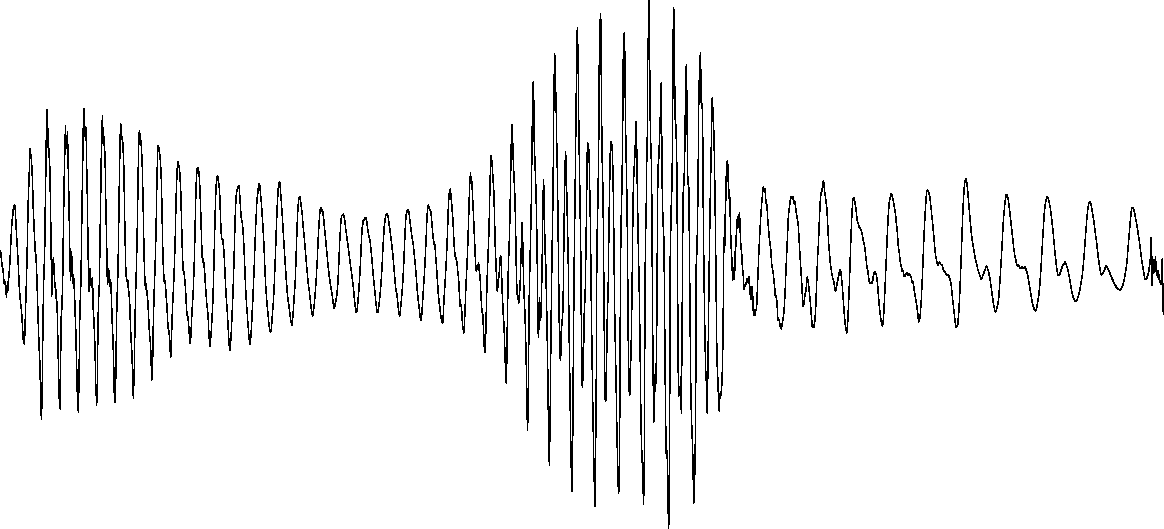
\includegraphics[width=.9\linewidth,height=.2\linewidth]{figs/waveform-zoomin.pdf}
    \caption{Zoomed-in waveform, showing 250ms. The frequency information is visible.}
    \label{fig:waveform-zoomin}
  \end{subfigure}
  \\
  \begin{subfigure}{\textwidth}
    \centering
    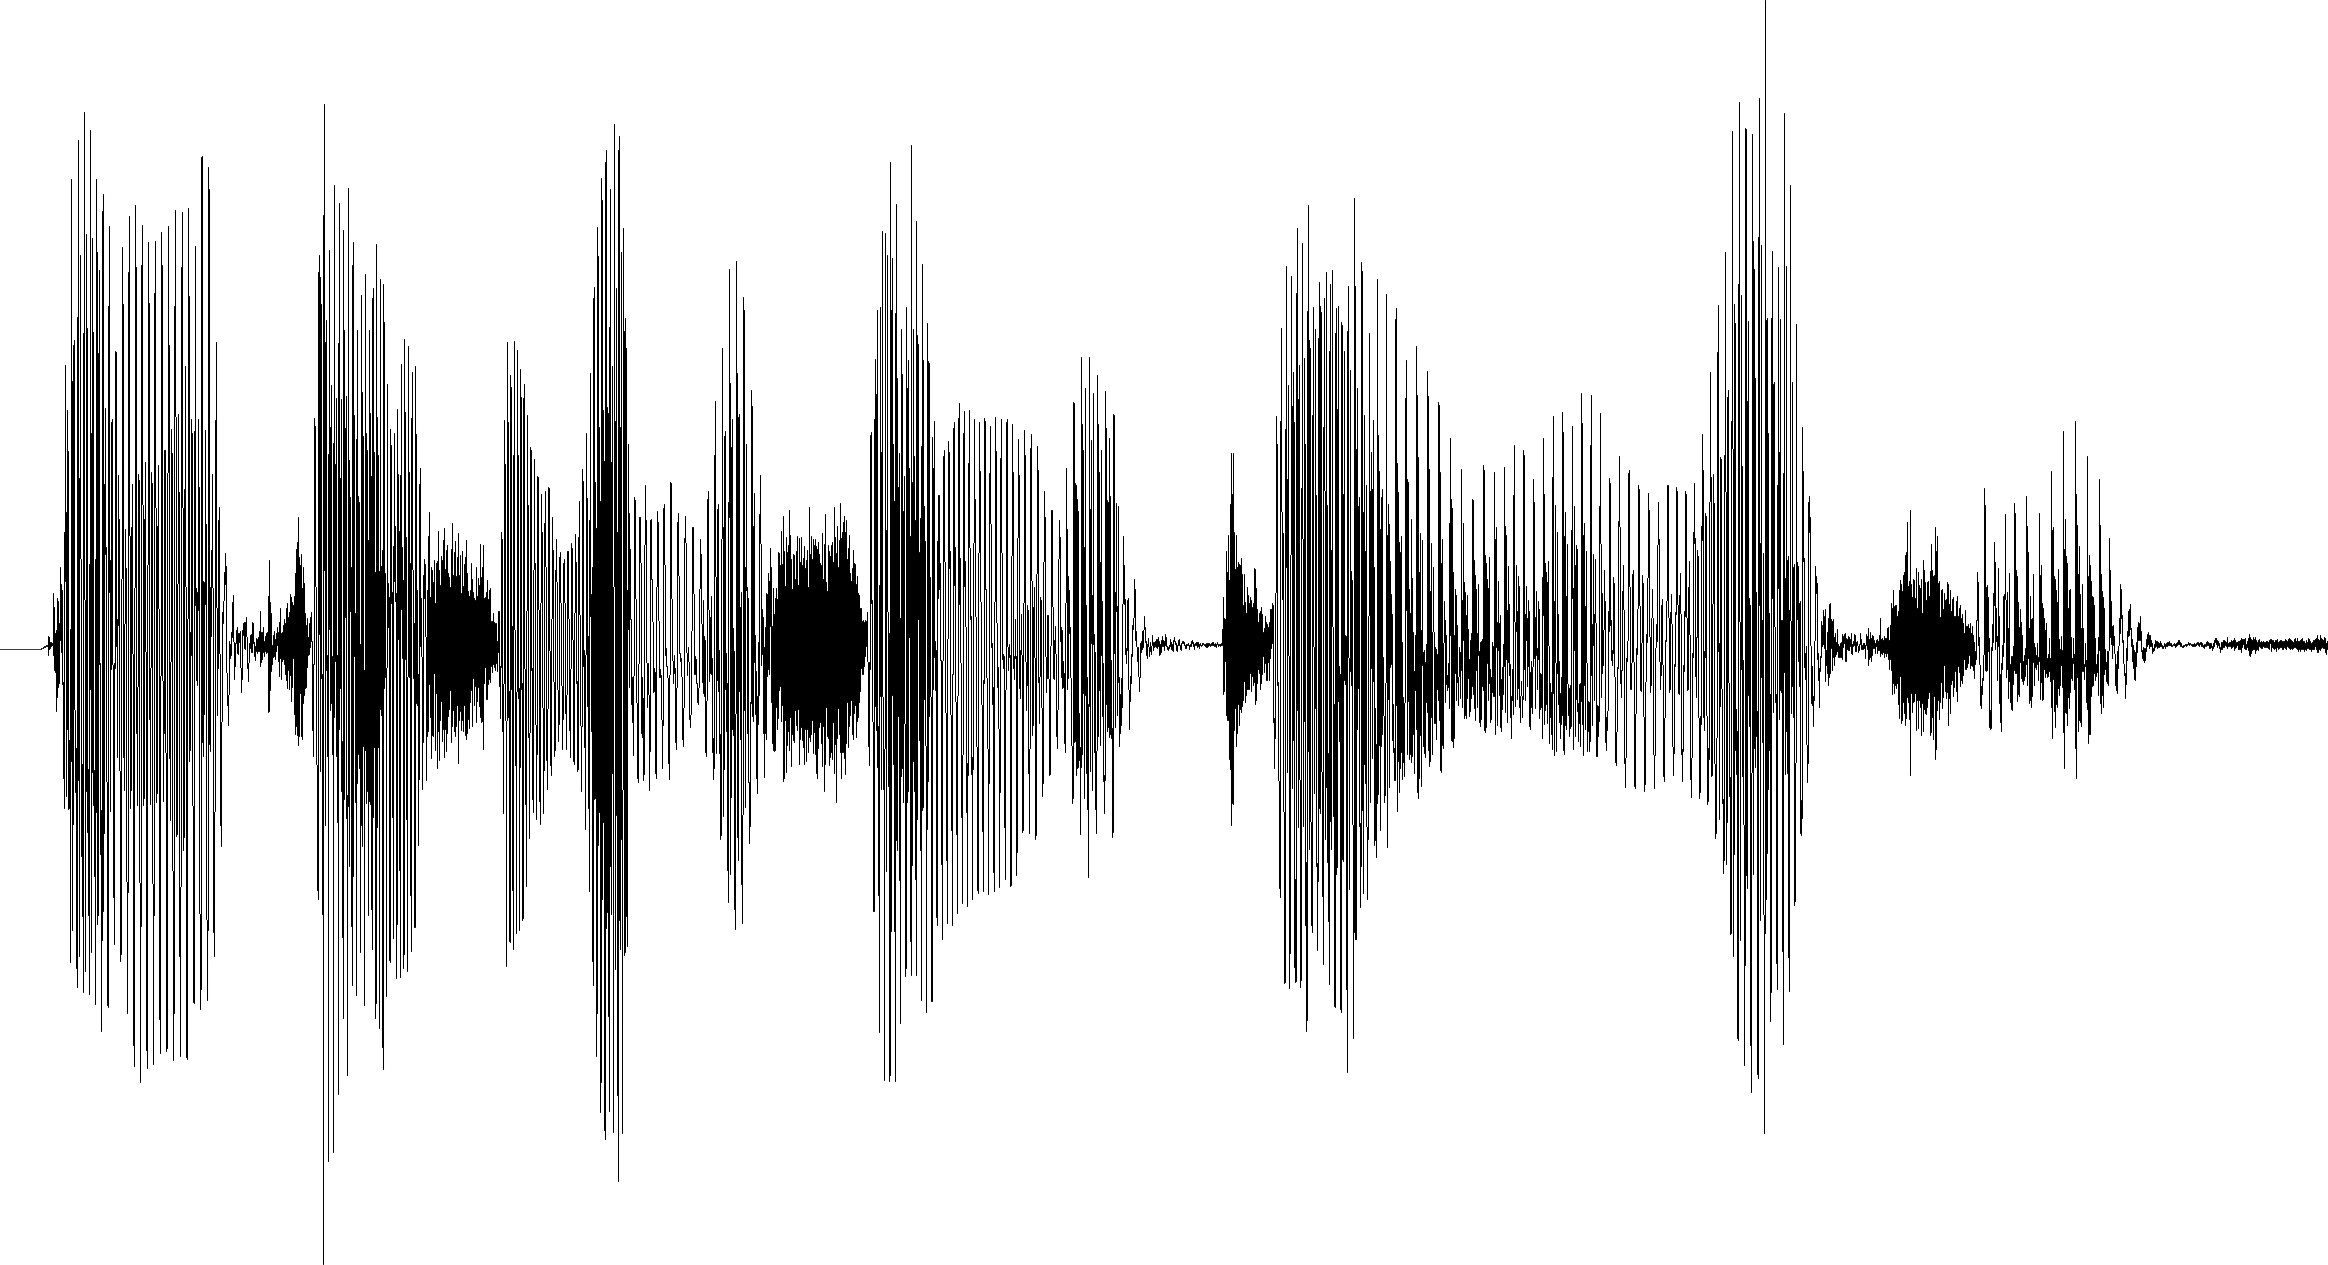
\includegraphics[width=.9\linewidth,height=.2\linewidth]{figs/waveform-zoomout.png}
    \caption{Zoomed-out waveform, showing 2500ms. The frequency information is not visible.}
    \label{fig:waveform-zoomout}
  \end{subfigure}
  \caption{Example audio waveforms of speech, demonstrating the effect of zoom on the visibility of frequency
  information}
  \label{fig:waveforms}
\end{figure}

An \textit{audio waveform} is a common graphical representation of an audio signal that is produced by plotting the
amplitude of an audio signal over time.
%Waveforms are a very simple audio visualisation technique, and arguably the most commonly used.
The curve of an audio waveform directly represents the pressure waves of sound.  The height of a waveform corresponds
to its amplitude, or volume. Lines that are closer together represent higher pitch sounds and lines that are farther
apart represent a lower pitch.
%As most natural sounds are composed of a multitude of frequencies, waveforms often have complex curves. 

% quiter/louder, deeper/higher pitch
% https://scienceaid.net/images/3/3d/sound.png

Waveforms have been used to visually represent audio content since the first digital audio workstations started to
appear \citep{Ingebretsen1982}.  Today, they are the default audio visualization used in all of the DAWs we surveyed.
The simplicity of the waveform makes it conceptually easy for users to understand and interpret the audio.  Waveforms
are relatively compact, so can be arranged vertically on top of each other to view multiple audio tracks
simulteneously. They are also computationally efficient to generate, as they are plotted in the time domain.
%TODO Can be used for a variety of tasks and applications

% loss of frequency information
Despite their popularity, waveforms display relatively little information about the audio.
Figure~\ref{fig:waveform-zoomin} shows a waveform that has been zoomed-in. At this scale, we can see the individual
cycles of the sound vibration, and the mix of frequencies that make up the sound.  However, when we zoom out, these
curves are compressed to the point where they are no longer visible.  Figure~\ref{fig:waveform-zoomout} shows a
waveform at a zoom level typical in audio production. At this scale, it is impossible to determine which frequencies
are present.  What remains is an ``amplitude profile'' that indicates the volume of the sound over time.

% readability of amplitude profile
Without frequency content, there is a limit to the amount of information waveforms can convey.  The amplitude profile
can be used to identify silences, peaks and the relative volume of different parts of the audio.  With experience, it
is possible to use the amplitude profile to distinguish different types of sounds. For example, the frequent short
periods of silence in Figure~\ref{fig:waveform-zoomout} indicate that this may be speech, because unlike music, speech
is broken up into words.

In order to be able to infer this information, users must learn what the amplitude profile of different sounds look
like. This would be a problem for novice producers, but not for professionals who work with audio on a daily basis.
However, the level of information that can be inferred is limited. For example, it is very difficult to use a waveform
to distinguish many important features, such as individual voices, or different styles of music.

We were interested in learning how audio waveforms affect the performance of audio editing tasks. However, despite the
popularity of waveforms, we could not find any studies that have attempted to measure the performance of audio
waveforms.

\subsubsection{Spectrograms}

\begin{figure}[t]
\centering
  \centering
  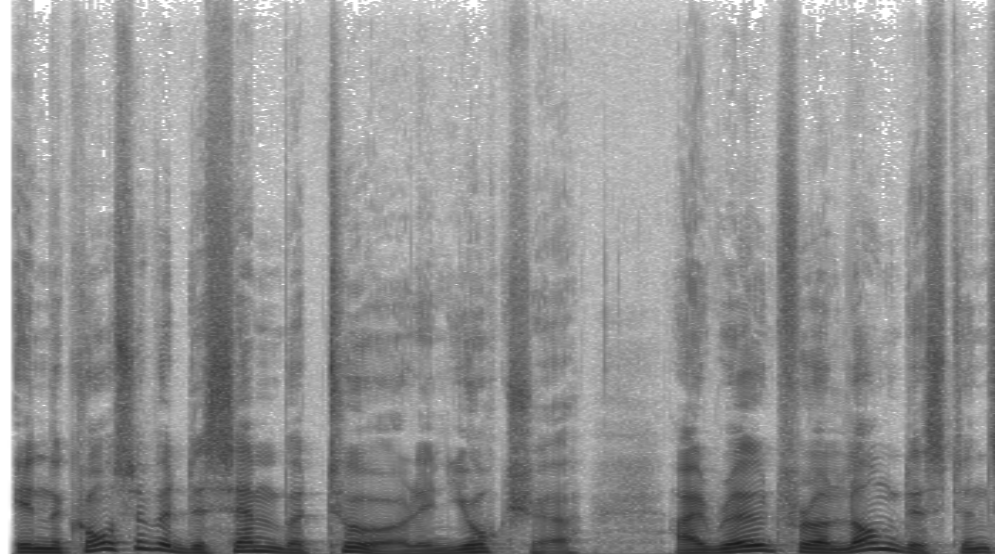
\includegraphics[width=0.8\linewidth]{figs/spectrogram-example.png}
  \caption{Example audio spectrogram of speech} 
  \label{fig:spectrogram-example}
\end{figure}

% WHAT IS A SPECTROGRAM?
A \textit{spectrogram} is a visual representation of the spectrum of frequencies in an audio signal over time. Higher
frequencies are displayed at the top of the spectrogram, and the energy of the signal is mapped to the brightness (or
sometimes colour) of the image. Figure~\ref{fig:spectrogram-example} shows an example spectrogram of a speech
recording.

Spectrograms clearly display the frequencies that make up the sound, and in what proportions.  When viewed at different
zoom levels, the frequency information is still visible, so it is much more robust to scaling than waveforms.  As
spectrograms are based on frequency analysis, they are more computationally expensive to generate than waveforms, but
this is rarely an issue with modern processors.

Like waveforms, spectrograms are conceptually very simple, and can be used for a variety of tasks and applications.
Spectrograms display a much higher density of information than waveforms, which can be used to infer more from the
audio. For example, \citet{Zue1986} found that expert users were able to use spectrograms to read individual phonemes
of speech. However, they also found that this was impossible for the average user to achieve.  Although spectrograms
present the data very clearly, users must still learn how to interpret the information.  

Reading spectrograms requires users to have a theoretical understand of audio frequencies and how they behave, such as
how a single pitch can be composed of many harmonics.  Although spectrograms display the energy present in each
frequency band, it is not apparent what the overall energy of the signal is at a given time.  Additionally,
spectrograms have a wide range of parameters that control how they are displayed, including window size and shape,
linear/non-linear frequency and energy scaling, min/max values and colour mapping.  This creates inconsistencies
between different spectrograms, which can make it difficult for users to move between software.  Waveforms don't have
as many parameters, so are much more consistent.

% HOW ARE SPECTROGRAMS USED? 

%The frequency scale in an audio spectrogram is usually presented on a logarithmic or Mel scale to give a better mapping
%of frequencies to the perception of pitch.

%Spectrograms are available in most audio editing software, but rarely used by default.

%TODO Can be used to edit frequencies like photoshop \cite{Boogaart2006}




%====================================================================================================================
\clearpage
\section{Semantic audio analysis}

Semantic audio analysis is the extraction of perceptual attributes from an audio signal, which is used to describe
sound in human-readable terms.  Semantic audio can be used to make sound recordings less ``opaque'' by allowing users
to interpret what is contained in the audio without having to listen to it first.  This approach can be applied to the
improvement of audio production interfaces. For example, \citet{Fazekas2007} enhanced a DAW to assist music producers
in navigating and editing their content by automatically segmenting music into verses and choruses.  We are interested
in how semantic audio analysis can be applied to user interfaces for the purpose of assisting the production of radio.

% different fields
In this section, we will provide an overview of the methods and applications of semantic audio analysis.  Semantic
audio brings together a wide variety of disciplines, including speech recognition, information retrieval, audio
analysis, signal processing, psychoacoustics, and machine learning \citep{Foote1999}. As such, we will only aim to
provide a brief overview of selected methods and applications that are relevant to radio production.  As the focus of
our research is on the pre-production of speech programmes, we will only cover methods and applications related to
speech content, which notably excludes the active field of music information retrieval \citep{Downie2008}.

% METHODS 
\subsection{Semantic audio features}\label{sec:features}

Semantic audio analysis is conducted by processing the audio using an algorithm to extract one or more semantically
relevant ``features''. This process known as \textit{feature extraction}.  Audio features are numerical representations
of certain properties of the audio, which are often categorised into low-level and high-level features
\citep[p.~31]{Fazekas2012}.  Low-level features include physical and perceptual properties, such as the energy and
spectral content of the sound.  High-level audio features correspond to more meaningful concepts, such as words and
people, or stuctural segments such as programmes or topics.  Many semantic audio algorithms use classification or
machine learning to map low-level features into high-level features. For example, in speech recognition, a
language model is used to map individual phonemes of speech into words and sentences.

%Feature selection and extraction are methods of reducing the dimensionality of a feature vector, either by choosing a
%combination of vector components that best describe the content (selection), or by translating the feature vector to a
%smaller vector while retaining as much information as possible (extraction).

%This process can be unsupervised where only the feature data is known (such as with principal component analysis), or
%supervised where the feature data has corresponding labels (such as with linear discriminant analysis).

%Canonical correaltion analysis (CCA) has been used to reduce the dimensions of features for speaker diarization
%\citep{Chaudhuri2009} and phonetic labelling \citep{Arora2014}, amongst other things. It is able to efficiently map
%features to a subspace and can be used with the kernel trick (known as KCCA) to support non-linear mappings.

%\citet{Chaudhuri2009} found that
%``CCA-based algorithms consistently provide better performance than standard PCA-based
%clustering methods''.

In this section, we will describe methods for semantic audio analysis that have been used in applications related to
radio production. We outline several feature extraction algorithms, and decribe some common methods that are used to
map them to high-level features.

%then classification/mapping/grouping/clustering
% low-level (frequencies) to high-level (words)
% map or group these features into semantically meaningful categories

% Extraction

There are a huge selection of semantic audio features that can be extracted from an audio signal. In this section, we
will describe a select few features that are touched upon in this thesis, to help illuminate the reader's understanding
of their origin.
%These only represent a small selection
%of the available features, but we have included them to give the reader an impression of how semantic audio works.

There are many different types of audio features that can be extracted. With music, rhythmic features are used to
extract the beats and tempo, and harmonic features are used to determine the notes and chords.  Speech is in some ways
a more complex signal to analyse, so more generic features are often used. Below we have outlined three types --
energy, temporal and spectral features.

%Prior to feature extraction, the audio signal is first segmented by time into equal-length chunks, known as
%``frames'', which are filtered using a window function. This enables the algorithm to 

%\paragraph{Feature learning}

%Traditionally, audio features were developed by hand for specific tasks. This was usually done by attempting to write
%an algorithm that calculated the properties of the sound that humans used to distinuish the categories in question.
%More recently, fuelled by an ever-increasing availability of computing power, research has had a much greater focus on
%automating this process.

%The above methods of reducing dimensionality are based on a relatively short information-rich feature vector that it
%suitable for the target application.  More recent research on feature development is focussed on automated learning of
%features using large labelled datasets.

%Deep learning is an increasingly popular method of learning features based on neural networks with large numbers (tens
%or hundreds) of hidden units. This line of research has been enabled by the increasing availability of large amount of
%processing power. When done properly, deep learning can produce the state-of-the-art in audio features, outperforming
%even the best hand-crafted features \citep{Hamel2010,Sigtia2014}.

%Such an approach requires a high-quality and very large labelled dataset, on which the success of the process depends.
%The nature of neural networks means that it is very difficult to interpret what the resulting features represent which
%isn't an issue when used as the input to a machine learning system, but would make it very difficult to map to a
%visualization. The objective of the deep learning process is to minimise a cost function rather than to maximise the
%link to human perception.

%Deep belief networks for feature learning \citep{Hamel2010}
%Deep neural networks for learning musical features \citep{Sigtia2014}


% low-level vs high-level?

\subsubsection{Energy features}

Energy features are based on the energy of the audio signal, and how it changes over time.  Similarly to audio
waveforms, energy features can be used to infer certain properties of the sound, such as whether it is likely to be
music or speech.  Calculating energy features is often computationally efficient, which makes them attractive for use
in real-time applications, or on large data sets.

A simple and popular low-level energy feature is \textit{root mean square} (RMS), which is calculated as the square
root of the mean square of the audio signal. RMS is commonly used in scientific work as a measurement of a signal’s
power.  The statistics of an audio signal's RMS value can be used as an effective classifier of music and speech, as
demonstrated by \citet{Ericsson2009} and \citet{Panagiotakis2005}.

RMS energy is also used as the basis for other features.  \textit{Low energy ratio} (also known as `silent interval
frequency' or `energy contour dip') is a measure of the number of RMS energy frames that fall below a threshold. It is
used for speech/music discrimination (SMD), and works by exploiting the fact that speech has freqent silent gaps between
words, wheras music does not. The threshold can be set as a fixed value \citep{Liang2005}, a function of a moving
average \citep{Ericsson2009} or moving peak value \citep{Saunders1996}.

\subsubsection{Temporal features}

Temporal features are based on statistics of the audio samples. These statistics are calculated in the time domain, so
like energy features, temporal features are computationally efficient.  A popular temporal feature is
\textit{zero-crossing rate} (ZCR), which is the rate at which a signal crosses the time axis. ZCR can be used as a
crude measure of pitch or the distribution of spectral energy.

Early work in SMD \citep{Saunders1996} identified that ``speech signals produce a marked rise in the ZCR during periods
of fricativity occuring at the beginning and end of words'', wheras music does not. This causes a bimodality in the
distribution of the ZCR, which can be detected by measuring its ``skewness''.
%The variance of ZCR has also been found to perform well for SMD \citep{Scheirer1997}.
\citet{Panagiotakis2005} also found that ``RMS and ZCR are somewhat correlated for speech signals, while essentially
independent for music'', and so the product of RMS and ZCR can also be used as a SMD classifier.

%ZCR also played a significant role in two steps of a five-step classifer \citep{Panagiotakis2005}. During silent
%intervals the number of zero crossings is null, so this was used to detect gaps between speech.

%A review \citep{Carey1999} of features for SMD found ZCR to perform least well, but did not consider the skewness,
%variance, or probability of null zero-crossings.

\subsubsection{Spectral features}

Spectral features decompose the audio signal into frequency bands to analyse the frequencies that are present in the
signal, and in what proportion.  This is commonly performed using a fast Fourier transform.

% Spectral centroid
\textit{Spectral centroid} is a measure of the ``centre of mass'' of the spectrum, calculated as the mean of the audio
frequencies, weighted by the magnitude of each frequency bin.  Audio with more higher frequencies than lower
frequencies has a higher spectral centroid value, and vice-versa.  Spectral centroid is a good predictor of the
perceived ``brightness'' of the audio, which can be used to distingish sounds of different timbre
\citep{Schubert2004}.

% What are MFCCs?
The \textit{cepstrum} of a signal is the power spectrum of the log of its power spectrum \citep{Noll1967}. The cepstrum
is a compact representation of how the frequencies in a signal change over time.  The Mel-frequency cepstrum is
calculated by spacing the frequency bands using the Mel scale \citep{Stevens1937}, which gives a better approximation
to the human hearing system. The audio features produced through this process are called \textit{Mel-frequency Cepstral
Coefficients}, or \textit{MFCCs} \citep{Imai1983}.
MFCCs are commonly used as a speech analysis tool, and have been successfully applied to SMD
\citep{Liang2005,Pikrakis2008,Pikrakis2006a,Sell2014,Wieser2014} and speaker segmentation
\citep{AngueraMiro2012,Friedland2009}.

%The mapping between MFCCs and semantic labels is usually complex, so is often used in combination with machine
%learning techniques.

%Friendland et. al. \citep{Friedland2009} found that enhancing the standard MFCC features with prosodic features, which
%measure the rhythm and intonation of speech, improved speaker diarization by 24\%.

%proposed enhancing the standard MFCC features with a set of long-term features
%representing prosody (the rhythm and intonation of speech). 52 candidate features were ranked using feature selection,
%which showed that ``the median and mean fundamental frequency are the best features, following by high formants (F4,
%F5)''. Inclusion of the top ten prosodic features improved the speaker diarization system by 24\%.

%% CLASSIFICATION
%\subsubsection{Classification}

%% Mapping/grouping/clustering/modelling
%% - machine learning
%% - clustering
%% - markov models
%% - GMMS

%HMM intro \citep{Rabiner1989}

\subsection{Applications}

Semantic audio analysis allows us to gain insights into the content of audio recordings without having to listen to
them. The techniques we described have already been used to tackle a variety of problems \citep{Foote1999}.  In this
section, we will present three applications of semantic audio analysis that have applications to radio production, and
outline their aim, methods and performance.

%\paragraph{Audio classification}
%\citet{Liang2005} divides audio streams into five classes: silence, noise, pure speech, speech over background sound
%and music. Four new features are proposed, including silence ratio, pitch frequency standard deviation, harmonicity
%ratio and smooth pitch ratio.

%Survey \citep{Duan2014}

\subsubsection{Speech/music discrimination}

\textit{Speech/music discrimination} (SMD) is the task of segmenting and labelling audio content into sections of
either music or speech.  Many SMD systems have been specifically developed for use with radio broadcasts
\citep{Saunders1996,Pikrakis2006,Pikrakis2008,Ericsson2009,Wieser2014} and television broadcasts
\citep{Seyerlehner2007,Sell2014}.  SMD systems have been successfully implemented using a variety of different
features, including low energy ratio \citep{Ericsson2009}, ZCR skewness \citep{Saunders1996}, spectral entropy
\citep{Pikrakis2006}, continuous frequency activation \citep{Seyerlehner2007,Wieser2014}, chromagrams \citep{Sell2014}
and MFCCs \citep{Pikrakis2008}.  \citet{Carey1999} compares the performance of some common SMD audio features.

Most SMD systems report high accuracy figures of 96\% and above, which shows that automatic SMD is likely to be useful
in real-life applications.  However, each system is evaluated using different data sets that are inconsistent in
content and length, which makes it difficult to compare them \citep{Pikrakis2008}.  \citet{Wieser2014} found that by
including a user-adjustible slider, the accuracy of their SMD system increased from 96.6\% to 100\%.

\subsubsection{Speaker diarization}
\textit{Speaker diarization} is the task of segmenting an audio recording into labelled segments that identify who
spoke when \citep{AngueraMiro2012}. With this task, the location of any speech content and number of speakers is
usually unknown. Speaker diarization has clear applications to the production of radio, where there are often multiple
people speaking in a single recording, and it is desirable to know where they are speaking without having to listen.

\citet{Tranter2006} and \citet{AngueraMiro2012} show that the vast majority of systems are based on clustering of
MFCCs, and that current research is focussed on the improvement of clustering algorithms and pre-processing stages,
rather than audio features. Most of the recent research has focussed on recordings of meetings, rather than broadcast
content.

%\citet{Foote1998} describes a video browser prototype that allowed the user to control this threshold value,
%using a slider in the user interface. Their prototype identified speaker turns, but did not attempt to match the
%identities of the speakers.

%Friendland et. al. \citep{Friedland2009} found that enhancing the standard MFCC features with prosodic features, which

\citet{AngueraMiro2012} found that the average error rate for speaker diarization systems was 11.6\% and 17.7\% for two
standard data sets. However, these data sets are based on microphone recordings of meetings, rather than broadcast
content.  \citet{Bell2015} conducted an evaluation of speaker diarization systems on television recordings of multiple
genres.  These results showed that the error rate was 47.5\%, which is considerably higher.  However, the evalation was
conducted across multiple recordings, which made the task of matching speakers more difficult.  A breakdown of the
results showed that most of the errors were misidentification of speakers, and that misidentification of speech
accounted for less than 8\% of the error rate.

Speaker diarization systems assign a unique identity to each speaker, but they do not attempt to identify who the
speaker is. \textit{Speaker recognition} is the task of identifying a person based on the sound of their voice
\citep{Doddington1985,Lee1999a}. Extracting metadata such as participant names and genders from radio content would
enable automated information searching and indexing \citet{Kinnunen2010}. Speaker recognition relies on access to a
database of trained speaker models, which represent people's voices. In radio, many of the contributors are from a
small pool of presenters, so it may be feasible to use speaker recognition techniques to detect their voices with
sufficient accuracy.

\citet{Raimond2014} introduced the \textit{BBC World Service Archive prototype}, which was an interface that used
automatic keyword tagging and crowd-sourcing to support the search and discovery of a large radio archive.
The interface used speaker diarization and speaker identification to help users navigate within individual radio
programmes. Figure~\ref{fig:bg-world-service-archive} shows an example of a radio programme that has been segmented
into five named speakers.

\begin{figure}[ht]
  \centering
  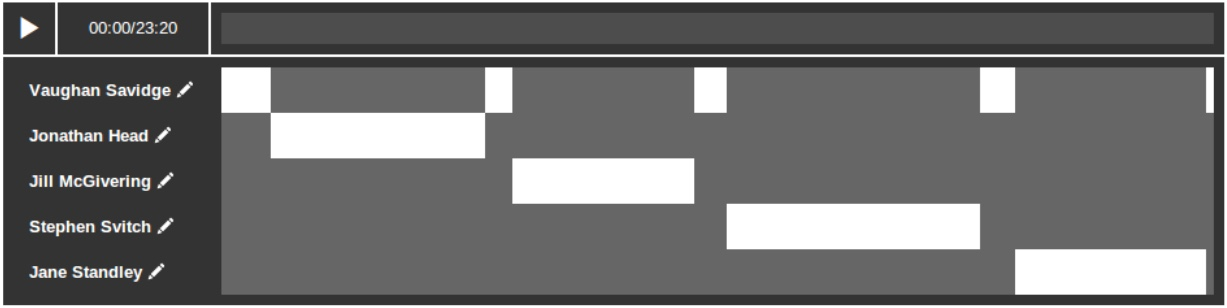
\includegraphics[width=\linewidth]{figs/world-service-archive.jpg}
  \caption{Speaker diarization and identification interface in the BBC World Service Archive prototype, from
  \citet{Raimond2014}}
  \label{fig:bg-world-service-archive}
\end{figure}


%Book \citep{Lee1999a}

\subsubsection{Automatic speech recognition}\label{sec:asr}

\textit{Automatic speech recognition} (ASR) can be used to automatically convert speech to text.  Modern ASR systems
can be broken down into two main stages \citep{Junqua1995}.  The ability to convert audio signals to text opens up many
possibilities in radio production, such as being able to navigate audio recordings through searching and skimming.
These opportunities are discussed in greater detail in Section~\ref{sec:background-transcripts}.

Modern ASR systems can be broken down into two main stages \citep{Junqua1995}. The first stage uses an acoustic model
to map the audio to a set of ``phonemes'' that make up the speech. In the second stage, a language model converts the
sequence of phonemes into words and sentences. Both the acoustic and language models are developed using machine
learning techniques to train the system based on recordings and transcripts of speech.  The success of an ASR system
depends on both how advanced the technology is, and the quality and fitness of the data that it is trained on.

% accuracy
Despite advances in the field \citep{Lee1999a}, ASR produces erroneous transcripts.  \citet{Bell2015} conducted an
evaluation of ASR systems on television programmes of various genres. Each system was judged by the proportion of
incorrect words, known as the ``word error rate'' (WER).  The mean average WER of the systems tested was 23.7\%,
however the variance across the programmes was high, with the WER varying from 10 -- 41\% across the 16 programmes.

%Speech alignment \citep{Bohac2013}
% can also be used with post-processing to conduct topic identification and segmentation

%=====================================================================================================================
% VISUALISATION
\clearpage
\section{Audio visualization}\label{sec:background-visualization}
Audio visualization is the task of mapping an audio signal to an image. The human visual system is capable of viewing
an entire image at once, and is adept at searching and skimming images. On the other hand, sound must be
consumed serially and over a period of time. Mapping sound to vision allows temporal information to be displayed
spatially, which can overcome some of the limitations of a time-based medium like sound.

We saw in Section~\ref{sec:background-daw} that audio visualization is already used in DAWs to help users navigate and
edit audio content.  However, we also saw that current audio visualizations are limited in what they can display.  For
example, waveforms only display amplitude information, much of which cannot be seen at typical zoom levels.  To
effectively navigate audio waveforms, users must interpret the shape of the visualization to infer whether it is what
they are looking for.  Although in many cases this can be learned, it requires cognitive load to process the images
into the desired information. It also means that novice users must be trained or gain sufficient experience to be able
to reach satisfactory performance levels.
%Audio visualizations can help overcome the contraints of having to consume audio content serially and in real-time.
%Most existing tools treat audio as a collection of digital samples, without much regard for the information contained
%in the audio.

Previous research has proposed a number of enhancements to current audio visualizations that aim to improve their
performance, such as by mapping semantic audio features to colour.  In this section, we start by looking at the
relationship between sound and vision, and considering the perceptual mappings between the two that already exist. We
then review techniques that have been previously used to process or enhance waveforms and spectrograms to make it
easier for users to navigate and edit audio recordings.

%TODO Mention Sonic Visualizer from \citet{Cannam2010}

%TODO Colour, size and orientation guide visual attention for visual search \citep{Wolfe2004}

%Semantic audio is the extraction of meaning from audio. Example applications of semantic audio are speech-to-text or
%music identification. This technology allows the computer to interpret the audio on the user's behalf in a way that is
%helpful for their situation, however the success of this is dependent on the performance of the audio analysis
%algorithm.

%Semantic audio visualisation is a two-stage process where the audio is first analysed to extract the semantic data,
%then the data is visualised. There are thousands of audio extraction and data visualisation techniques that could
%be combined to create various audio visualisations. The interaction of these two parts, and the context of the
%application, is important in the sucess of semantic audio visualisation. 

%Visual systems can be used to complement audio interfaces, as they are able to address the key challenges of sound.

%In modern society, screens for displaying visual content are widely available.


%Academic research into audio analysis and audio interfaces tends to concentrate on fully automated systems
%\citep{AngueraMiro2012}, navigation of large audio collections \citep{FontCorbera2010} or navigation interfaces based
%on skimming \citep{Arons1997} and scrolling \citep{Lee2007}. Although there are examples of audio visualization from
%the world of academia, it is much more popular in the context of art \citep{Armitage2012}, with excellent examples such
%as Quayola's Form--Sound--Abstraction\footnote{\url{http://www.quayola.com/work/form-sound-abstraction/}} work.


%In a world of `big data', data visualization is becoming an increasing popular subject. Visualization techniques have
%been applied to audio content for a
%variety of applications including accessibility \citep{Ho-Ching2003}, browsing
%large databases \citep{FontCorbera2010}, browsing small databases \citep{Yoo2011} and musical training
%\citep{Ferguson2005} amonst others.

%The development of good visualizations lies somewhere between science and art.
%Tufte's seminal work on good practice \citep{Tufte2001} gives solid guidance on
%creating elegent and unbiased visuals, and Wolfe and Horowitz \citep{Wolfe2004}
%tell us which properties of vision are most critical for visual search.
%However, putting these together in the context of audio requires a certain
%amount of creativity.

%This project focusses on `visualization of time-oriented data', a good overview
%of which can be found in a Springer book of the same name \citep{Aigner2011}.
%The rest of this section will look at examples of time-oriented visualization
%of audio, grouped by the most common visualization techniques.

\subsection{Crossmodality}\label{sec:crossmodality}
To be able to represent audio visually, we must map auditory properties to visual properties.  When attempting to link
sound and vision, it is desirable to create a mapping that is coherent and makes sense to the user.  By creating an
audio visualisation that ``looks likes it sounds'', it might be possible for users to comprehend the sound without
having to listen to it.

\textit{Crossmodal perception} is a term used to describe interaction between the different senses.  Previous work has
shown that there are perceptual mappings between auditory and visual stimuli that are experience by most of the
population. These could be exploited to aid the navigation and editing of audio recordings.

\begin{figure}[ht]
\centering
  \centering
  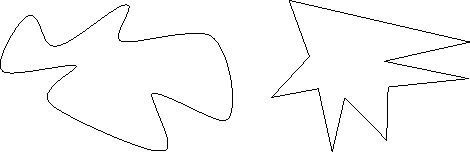
\includegraphics[width=0.8\linewidth]{figs/bouba-kiki.pdf}
  \caption[Demonstration of crossmodal perception.]{Demonstration of crossmodal perception. \citet{Ramachandran2001}
  found that 95--98\% of the population assigned the names `bouba' and `kiki' to these shapes in same order. See
  footnote \ref{bouba-kiki-answer} on page \pageref{bouba-kiki-answer} for answer.}
  \label{fig:boubakiki}
\end{figure}

The ``bouba/kiki effect'' is a demonstration of cross-modal mapping between sound and vision, originally discovered in
an experiment by \citet{Koehler1929}.  Participants were shown two abstract shapes, shown in
Figure~\ref{fig:boubakiki}, and asked to assign the name `bouba' to one, and `kiki' to the other\footnote{K\"ohler used
the words `baluma' and `takete' in the original experiment, but the result was the same.}.  \citet{Ramachandran2001}
found that 95--98\% of the population gave the same answer\footnote{\label{bouba-kiki-answer}The vast majority of
participants chose to name the sharp, pointy shape on the right `kiki' and the curvy, rounded shape on the left
`bouba'.}. This is an example of just one audio-visual mapping that is common amongst the population.

%\citep{Hubbard1996} did some work to determine which sounds related to which visual properties

%These audio-visual associations are not just higher-level constructs that our
%concious brain creates, they affect the brain at the very lowest level even
%with only brief exposure to bimodal stimuli. Zangenehpour et. al.
%\citep{Zangenehpour2010} used a PET-CT scanner to measure blood flow in the
%brain during exposure to audio and visual stimuli. ``When presented with only
%the auditory or visual components of the bimodal stimuli, na\"{i}ve subjects
%showed only modality-specific cortical activation, as expected.  However,
%subjects who had previously been exposed to the audiovisual stimuli showed
%increased cerebral blood flow in the primary visual cortex when presented with
%sounds alone.''

\begin{table}
\centering
\begin{tabular}{l l}
\hline
\textbf{Link} & \textbf{Direction} \\
\hline
Loudness/brightness  & louder=brighter \\
Pitch/elevation & higher=higher \\
Pitch/size & higher=smaller \\
Loudness/size & louder=bigger \\
Pitch/elevation & higher=higher \\
Pitch/spatial frequency & higher=higher \\
\hline
\end{tabular}
\caption{Audio-visual mappings supported by strong evidence, from \citet{Spence2011}}
\label{tab:crossmodal}
\end{table}

\citet{Spence2011} presented a review of psychology experiments that attempted to find cross-modal links in the human
brain, including audio-visual mapping.  He found that there was strong evidence for six audio-visual mappings, shown in
Table~\ref{tab:crossmodal}.
%There are two common types of test methods used to discover these links -- `speeded' and `unspeeded'.  In `speeded'
%tests, participants are tasked with classifying an audio/visual stimulus and their reaction time is measured. When the
%auditory and visual stimuli are `congruent' (perceived to be similar), then their reaction times are quicker. In
%`unspeeded' tests, visual and audio stimuli are presented very quickly, one after the other, and participants are
%asked to select which stimulus came second. When the stimuli are congruent, participants find it more difficult to
%work out the order of presentation.
These findings were supported by \citet{Tsiros2014}, who attempted to generate images to match different sounds and
measured their success through a user study. In addition to confirming the strong links between loudness/size and
pitch/elevation, he found weaker links for pitch/colour, dissonance/granularity, and dissonance/colour complexity.

%used a different approach to measure audio-visual crossmodality by using audio visualization
%techniques.  Three audio recordings were used -- a violin, recording of wind noise and impact sound event. For each,
%images were manually created which used different combinations of audio-visual mappings (e.g. dissonance $\to$ texture
%granularity). Participants were played an audio clip and shown an image and were asked whether they are similar or not,
%and to what degree (on a scale of 0--100).

%Tsiros confirms the results revealed by previous studies [7], [15], [19] which found strong relationships between the
%audio-visual feature associations of size – loudness, pitch – vertical position, and weaker relationships between
%color – pitch, texture granularity – sound dissonance and color complexity- sound dissonance

%Additional work from \citet{Marks2003} suggests that cross-modal interaction is a result of late-stage cognitive
%processes.

%Artwork that used synaesthesic style mapping for music to colour \citep{Armitage2012}

%Relationship between pitch and colour \citep{Datteri2004}

%Cross-modality can even be measured in the visual cortex using a PET scanner \citep{Zangenehpour2010}

%Vision and audition are physiologically separate, but idential in many respects
%\citep{Tsiros2013}.

Current audio visualizations exploit some of these cross-modal mappings. For example, waveforms map loudness to size,
and spectrograms map loudness to brightness, and pitch to elevation. However, this previous work shows that there are
many more links between sound and vision that have yet to be fully exploited by audio visualizations.

\subsection{Waveforms}

The audio waveform is commonly used by most DAWs and other audio software as a visualization of an audio signal.  As
such, users are very familiar with navigating audio content using waveforms, and many have learned how to read the
shapes of the waveform to read useful information about the audio. Enhancing waveform, by either processing it or
adding additional information to it, could allow users to navigate and edit audio content more efficiently whilst
retaining this familiarity and using the skills they have developed.  We identified two main approaches that have been
used to enhance waveforms -- scaling and colour.

\subsubsection{Scaling}
The scale at which a waveform is viewed is crucial to its effectiveness. There are two axes with which the scale is
controlled using horizontal and vertical zoom.  Horizontal zoom adjusts the time period that is viewed, which affects
the visibility of the frequency information.  Vertical zoom adjusts the amplitude range that is viewed, which affects
the visibility of the amplitude profile.

One very simple technique for improving waveform readability is to automatically scale the vertical zoom to match what
is visible on the horizontal timeline.  However, if the scale of the waveform constanstly shifts, there is no reference
level by which to compare the amplitude of the audio.  The solution proposed by \citet[p. 39]{Goudeseune2012} was to
overlaying a dimmed version of the scaled waveform on top of the normal waveform. This allowed users to simultaneously
judge the level whilst being able to see the detail of the amplitude profile.

Frequency information is useful for understanding the timbre of an audio signal. When viewed at the right scale, this
is visible in a waveform, but at typical horizontal zoom levels, this information is lost. \citet{Loviscach2011}
proposed a novel solution to this problem called the \textit{quintessence waveform}. This approach used extreme pitch
shifting to preserve the character of the waveform at different scales.  This works well for repeating monoaural sounds
-- for example, a sine wave would be identifiable as a sine wave at every zoom level.  However, typical real-life
applications use complex polyphonic audio, which would not benefit from quintessence waveforms as there is no repeating
signal that could be displayed.

%\begin{figure}[p]
  %\centering
  %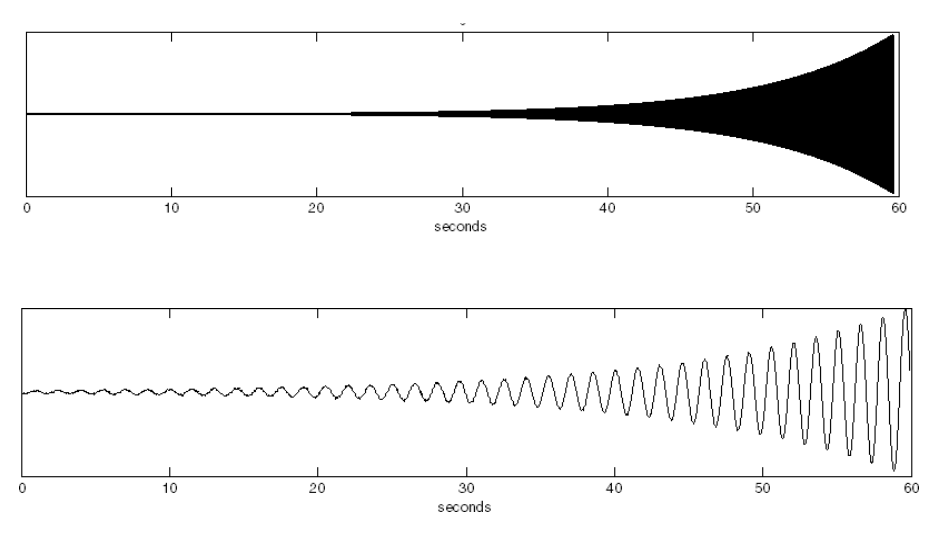
\includegraphics[width=0.95\linewidth]{figs/quint.png}
  %\caption{Above: Normal waveform, below: quintessence waveform, source: \citep{Loviscach2011}}
  %\label{fig:quint}
%\end{figure}

\citet{Gohlke2010} proposed five novel ideas on how to improve multi-track DAW displays, including techniques for
saving screen space by overlaying and stacking waveforms. One of these proposals was for a lens-like view, which
magnified the area of the waveform around the current playhead position. This allowed users to simultaneously view the
waveform at two different scales -- an overview of the audio waveform and a detailed local view. This concept has the
potential to display frequency information in regions of interest, and help make more precise audio edits without
adjusting the overall zoom level.

%waveform tracks can vertically overlap by 25\% without dramatically affecting display quality
%waveforms are mostly symmetrical, so by discarding one half the overlap can be increased to 50\%
%stack graph for contribution of each track to perceived loudness

\subsubsection{Colour}
The use of colour is a simple and effective way of adding additional information to a waveform.  However, many DAWs use
waveform colour to distinguish or label audio clips, and most others have monochromatic waveforms.  Previous research
has experimented with mapping semantic audio features to colour, using either pseudocolour or false colour.

\textit{Pseudocolour} is a method of mapping a scalar value to a colour gradient \citep{Moreland2009}, an example of
which is thermal imaging cameras.  Colour gradients are composed of at least two colours (e.g. blue to red) or a
spectrum of colours (e.g. a rainbow).  Pseudocolour allows values to be mapped to colours that might be perceptually
relevant (e.g. green/red for good/bad).  It can emphasize small variations between values by using a full spectrum,
pick out high/low values using non-linear gradients, or categorize values using stepped gradients.  However, as
pseudocolour can only represent one dimension, it does not make full use of the available colour space.

\textit{False colour} is the mapping of multiple values to the dimensions of a colour space. Commonly, three values are
mapped to red/green/blue (RGB) colour space. Other colour spaces can be used, such as hue, saturation, value (HSV),
which better matches human perception of colour. Hue means colour on a rainbow, saturation means lack of grayness, and
value means brightness. The advantage of this method is that it can make full use of the available colours.  On the
other hand, it can be challenging to select three values and map them to colour in a way that is perceptually relevant
and understandable.

\citet{Rice2005} presented \textit{Comparisonics}, which uses pseudocolour to map the frequency content of an audio
signal to a colour spectrum.  Comparisonics was designed for identifying timbrally distinct sounds and they claim that,
with training, it can be used to identify certain sound effects.  Their technique maps low/mid/high frequencies to
blue/green/red colours, respectively, using an unpublished algorithm.  Comparisonics has since been integrated into the
\textit{Scratch LIVE} DJ software from Serato Audio Research, where it was used to distinguish between different drum
noises, such as bass kicks, snares and high-hats.

A very similar system was implemented in the audio clip sharing website \textit{Freesound} \citep{Akkermans2011} to
help users quickly find and compare sound effects and music clips.  They used pseudocolour to map the ``spectral
centroid'' of the audio to a colour gradient.  Spectral centroid is the weighted mean of the frequencies of a signal
\citep[p. 10]{Smaragdis2009}, so a low value indicates the presence of mostly low-frequency sound and vice-versa.

\citet{Loviscach2011a} used pseudocolour to enhance the navigation of speech. The ``zero-crossing rate'' of the audio
was mapped to a red/green/blue colour spectrum to help distinguish between different phonemes (e.g. ``oo'' or ``s'').
The zero-crossing rate is the frequency with which an audio signal switches between a positive and negative value
\citep[p. 37]{Zhang2010}, which is a crude measure of the primary frequency of the audio.

\citet{Tzanetakis2000} used false colour to create a visualisation technique known as \textit{Timbregrams}. Their aim
was to ``use color perception and the pattern recognition capabilities of the human visual system to depict timbral and
temporal information''.  Their implementation extracted a large vector of common audio features, then used principal
component analysis to reduce the size of the vector whilst retaining 80\% of the variance in their data.  They mapped
the first three principal components of the feature to RGB or HSV colour space.  They found that the RGB colour space
was more uniform and aesthetically pleasing, but that the HSV colour space had better contrast at segmentation
boundaries. When using RGB, speech, classical music and rock could easily be distinguished as they appeared as light
green, dark blue and dark green, respectively. Tibregrams were later used to colour a waveform in a basic audio editor
\citep[p. 253]{Tzanetakis2001}.

\citet{Mason2007} used false colour to assist radio listeners in navigating recently-broadcast material. They mapped
three empirically-chosen audio features to RGB colour space. The authors reported that the system was successful at
indicating the location of music within speech content, and highlighting low-bandwidth material such as phone calls.
The authors proposed that the system could be also be applied to other applications such as segmentation of radio
programmes for re-editing into podcasts.

%\begin{figure}[p]
%\centering
%\begin{subfigure}{\textwidth}
  %\centering
  %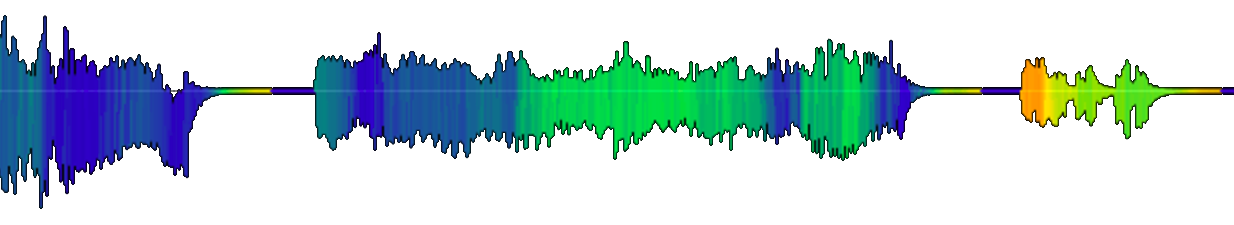
\includegraphics[width=\linewidth]{figs/freesound2.png}
  %\caption{Freesound (\url{freesound.com})}
  %\label{fig:freesound}
%\end{subfigure}\\%
%\begin{subfigure}{\textwidth}
  %\centering
  %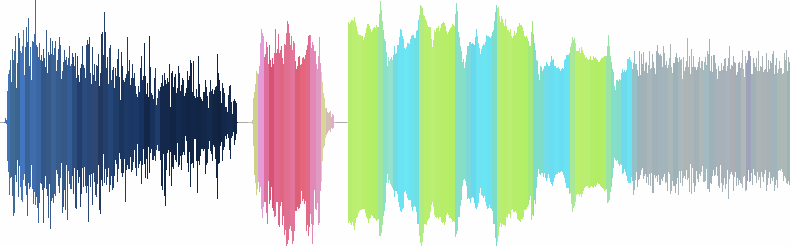
\includegraphics[width=\linewidth]{figs/rice.png}
  %\caption{Comparisonics \citep{Rice2005}}
  %\label{fig:rice}
%\end{subfigure}
%\caption{Examples of pseudocolour (\ref{fig:freesound}) and false colour
  %(\ref{fig:rice}) applied to colourising an audio waveform}
%\label{fig:colourvis}
%\end{figure}

%False colour has also been used for navigating and summarizing extremely long recordings. \citet{Towsey2014} mapped
%three spectral features to RGB colour for visualizing almost a year of environmental recording.
%Figure~\ref{fig:towsey} shows the recordings from March until October, with each line representing one day.  The
%visualization reveals the change in time of the dawn and evening choruses throughout the year, amongst other things.

%\begin{figure}[p]
  %\centering
  %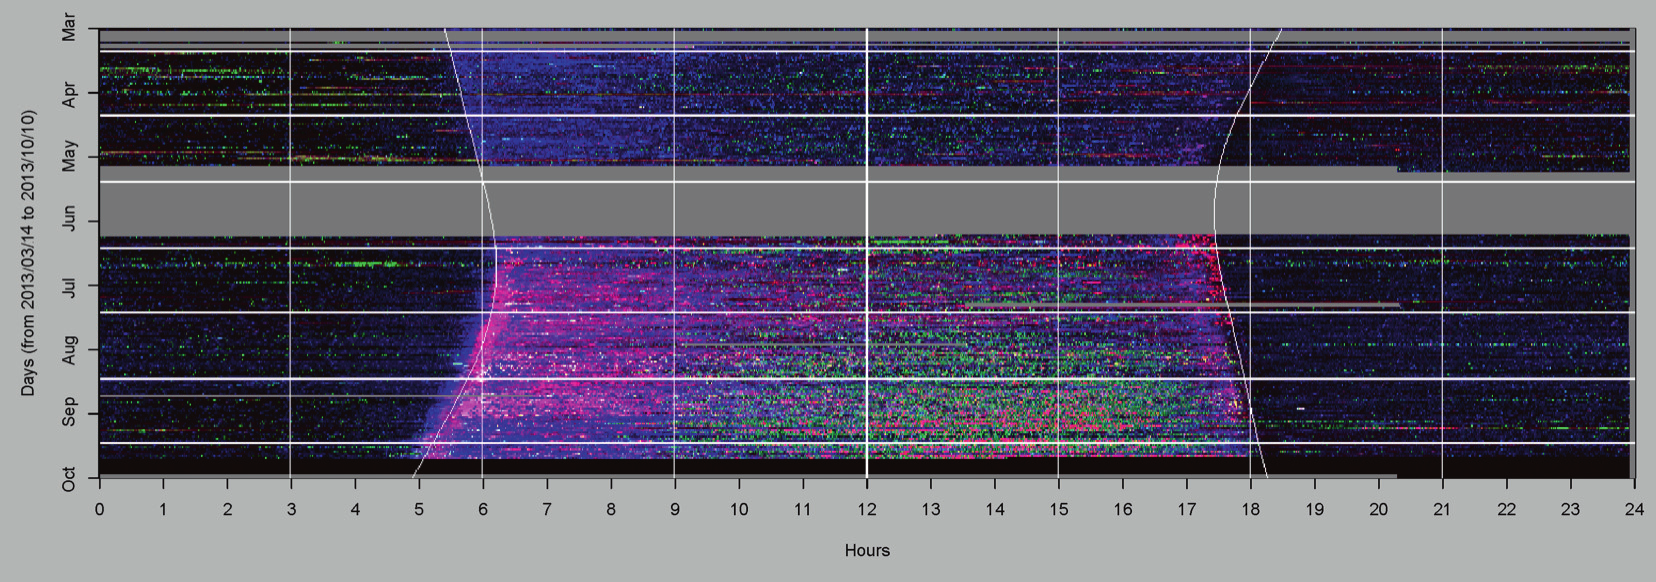
\includegraphics[width=0.95\linewidth]{figs/towsey.png}
  %\caption{False colour visualization of environmental recordings, with each line representing one day. Missing data is
    %shown in grey.
    %\citep{Towsey2014}}
  %\label{fig:towsey}
%\end{figure}

\subsection{Spectrograms}

Spectrograms display the amplitude of audio frequency over time. Unlike waveforms, the frequency information is visible
at all zoom levels, which makes them much more robust. They display so much information that, with sufficient training,
it is possible to read speech using a spectrogram \citep{Zue1979,Zue1986}.  However, despite these advantages, audio
waveforms are much more widely used than spectrograms in audio production.

%\citet{Gohlke2010} proposed a
%thresholded spectrogram overlaid with different colours for each track to minimuse spectrotemporal overlap and masking

\citet{Lin2012} introduced a method of filtering spectrograms to visually emphasize non-speech events in long audio
recordings. The filtering was done using an ``image saliency algorithm'' that detected differences in the intensity and
orientation of the spectrogram image. This \textit{saliency-maximized spectrogram} was integrated into an audio
navigation interface called \textit{Timeliner} \citep{Goudeseune2012}, which displayed the spectrogram alongside a
waveform. \citet{Lin2013} describes an evaluation in which 12 novice participants used Timeliner to find sound effects
hidden in meeting room recordings using both saliency-maximized and normal spectrograms. The results show that
saliency-maximized spectrograms significantly outperformed normal spectograms.
Filtering spectrograms shows promise as a way of detecting unusual events, however it is unclear how useful this sort
of application would be in the context of radio production.
%A user study of Timeliner for audio event detection \citep{Hasegawa-Johnson2011} Uses false colour to map min, mean
%and max values to the HSV colour space

%\begin{figure}[ht]
  %\centering
  %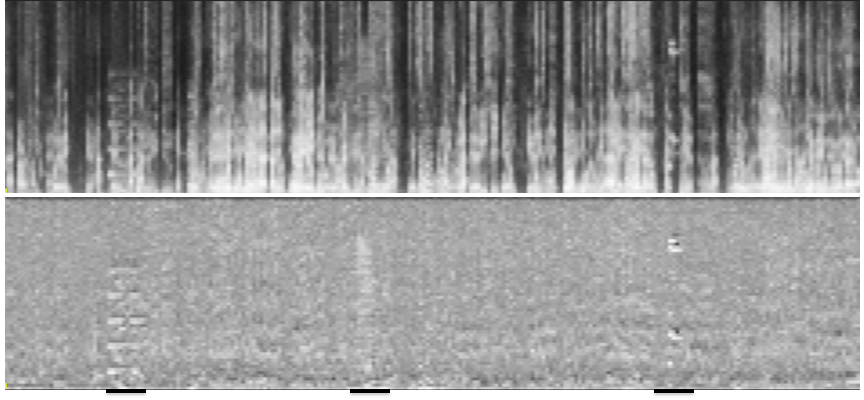
\includegraphics[width=0.95\linewidth]{figs/spectrogram-salience.png}
  %\caption{Top: A normal spectrogram; Bottom: A salience-maximised spectrogram with target events marked using black
    %underlines}
  %\label{fig:timeliner}
%\end{figure}


% Could use image synthesis \citep{Levkowitz1991}

%\clearpage
%\section{Speech segmentation}

%Waveforms and spectrograms provide a direct mapping of sound to vision, which is then interpreted by the user. The
%benefit of this approach is that it can be used for a wide variety of tasks with any type of content.  The downside is
%that the user must learn how to read these visualizations, and view them at an appropriate scale.

%With many audio recordings, the content can be divided into logical groupings that could help the user navigate the
%recording. For example, a ``magazine-style'' radio programme is made up of several pieces on different topics. Being
%able to view what those topics were, and where they occured in the programme, would assist listeners in navigating to
%a topic of interest.

%Semantic audio analysis techniques have been widely used to classify and segment audio into a range of logical
%categories. These are often combined with data visualization techniques \citep{Aigner2011} to create novel user
%interfaces that aid the navigation and editing of audio content.

%We have divided these segmentation techniques into two broad categories: classification, where audio is segmented by
%the character of the audio (speech, music etc.), and topic summarization, where the audio is segmented by its content.

%\subsection{Classification}

%Audio can be divided into human-readable segments using semantic audio analysis techniques.  Semantic audio analysis
%typically operates in two main steps: dividing an audio file into sematically meaningful segments, then grouping these
%segments into semantically meaningful categories \citep{Lu2009,Zhang2010}. These categories can be chosen to match the
%application being targeted. For example, a radio broadcast might be divided into speech, music, speech mixed with music
%and applause.

%This semantic audio segmentation has applications to audio editing \cite{Avdelidis2007}.

%\subsubsection{Speech/music discrimination}
%Speech-music discrimination (SMD) is the task of segmenting an audio recording and labelling those segments as either
%speech or music.
%Previous research into automated SMD has often targeted recordings of radio broadcasts
%\citep{Goodwin2004,Wieser2014,Saunders1996,Pikrakis2008,Pikrakis2006a}.
%%Clustering is a task in which comes naturally to humans, but machines often struggle with.




%\subsubsection{Speaker diarization and identification}
%\textit{Speaker diarization} is the task of segmenting a speech recording according to speaker identity, which is used
%to answer the question ``who spoke when?'' \citep{AngueraMiro2012}. Segments are given a unique label for each speaker,
%but the identity of the speakers is unknown.  \textit{Speaker identification} is the task of identifying the person who
%is speaking based on the sound of their voice.

%%Speaker identification with crowd-sourcing achieved 85\% precision and a 43\% recall

%which used speaker diarization and
%identification to facilitate navigation of radio programmes. The prototype relied on crowd-sourcing to add the speaker
%names, which then populated a central database of speaker identities.

%Segmentation algorithms often use a threshold value to configure their sensitivity. In the case of speaker diarization,
%a low threshold would increase the recall and reduce the precision. For example, more speaker turns would be detected,
%but some may be incorrect.  This threshold is often set to minimise a cost function, which balances the precision and
%recall.




\clearpage
\section{Semantic speech interfaces}\label{sec:background-transcripts}

Writing is widely used to record speech, in a process known as ``transcription''. Transcripts can be used to record
exactly what somebody said, and the transcript text can be read, copied, shared, skimmed and searched using a variety
of tools, such as word processors, or on paper.  \citet[p.~133]{Hausman2012} notes that radio producers currently
``cut, paste and copy sound files much the same way we use a word processor to manipulate words, sentences and
paragraphs''.  In this section, we will see how transcripts can be used as an interface to aid the navigation and
editing of speech recordings.

% transcripts can increase the navigation speed
\subsection{Transcript generation}\label{sec:transcript-generation}
Transcript are often written manually, either using pen and paper or a word processor. Based on the author's informal
discussions with radio producers, it can take them between 2 and 5 times the length of recording to transcribe
the speech, and is a slow and tedious process. Producers can save time by only transcribing the most salient words, but
this makes the transcript much less readable, particularly to others who haven't heard the original recording.
Alternatively, producers can use a third-party to transcribe the speech on their behalf, but this slow and expensive.
For example, \texttt{rev.com} charges \$1 per minute for a 12-hour
turnaround\footnote{\url{https://www.rev.com/transcription}, accessed 11/12/2017}.

% two types: manually written (perfect, but expensive and slow) or automatic (erroneous, but fast and cheap)
% comparison?
As we saw in Section~\ref{sec:asr}, ASR can be used to convert speech to text automatically.  ASR is quicker and
cheaper than manual transcription.  ASR also produces accurate timestamps for each word, which can be used to precisely
navigate and edit the audio, but word-level timestamps can also be added to manually-written transcripts using speech
alignment \citep{Griggs2007,Bohac2013}.  ASR transcripts don't include letter capitalization or punctuation, but this
can be estimated and added using post-processing.

Erroneous transcripts reduce listener comprehension \citep{Stark2000,Vemuri2004} and increase the time it takes to
search audio content \citep{Ranjan2006} and correct errors \citep{Burke2006}.  However, despite these errors, ASR
transcripts provide a highly effective tool for browsing audio content as users can visually scan the text to focus on
regions of interest, known as ``strategic fixation'' \citep{Whittaker2007}.

%\citet{Vemuri2004} conducted a user study of 34 participants and measured their comprehension of short audio clips when
%presented with both perfect and auto-generated transcripts.  The results show that subject comprehension of audio
%presented with a perfect transcript (C1) was found to be better than an automatically-generated transcript.
%completely wrong transcripts aren't worse than no transcript

%\citet{Ranjan2006} studied the performance of 13 participants in an audio search task with varying levels of
%transcript quality. The results showed that the mean search time descreased as the transcript quality increased.

%\citet{Burke2006} found that higher quality transcripts required users to listen less to complete a correction task.

%Automatic speech recognition technology makes it possible to extract partially accurate transcripts of speech
%recordings.  A number of researchers have experimented with using these transcripts to enhance interfaces for
%interacting with audio content.
%\subsection{Navigation}

% navigation with transcripts

\subsection{Transcript navigation}
Transcripts have previously been used by several systems as an interface for improving the navigation of speech-based
content such as news reports and voicemail messages. 
One of the first such systems was \textit{NewsTime} from \citet{Horner1993}, which used transcripts to aid the
navigation of audio news stories.  For television news, closed captioning was aligned the audio to provide an accurate
transcript with word timings.  NewsTime included several additional features including searching by keyword, segmenting
the transcript by story and speaker, jumping to the next or previous speaker/story, and categorizing stories into one
of seven common topics. There were no reported user studies of NewsTime.

\textit{SCAN} \citep{Whittaker1999} was an interface designed to support retrieval from speech archives. It used ASR transcripts
to allow users to search for keywords and visually search the recording by reading the transcript.  In a user study of
12 participants, the transcript was found to support navigation by reducing the listening time needed to complete
information retrival tasks. Participants rated the transcript as easier and more useful with the transcript than
without.  SCAN was further developed into \textit{SCANMail} \citep{Whittaker2002}, an interface designed for interacting with
voicemail.  It added a number of features including paragraph segmentation and the ability to seek to a point in the
audio recording by clicking on a word in the transcript. The results of a user study of eight expert users showed that
the transcript display enabled users to visually scan the content of recordings to quickly extract information and
judge which parts were relevant, without having to play the audio.
%SCANMail did not include editing capabilities

\subsection{Semantic speech editing}\label{sec:background-semantic-editing}
In addition to supporting the navigation of speech recordings, transcripts have also been used as a method of editing
speech content. The first of these was the `Large Interactive Display System Wave Speech Editor', or
\textit{LIDSWSEdit}, from \citet{Apperley2002}, which used ASR transcripts to allow users to navigate and edit lecture
recordings.  Any edits made to the transcript were correspondingly applied to the underlying audio recording, known as
``semantic speech editing''. Users could re-arrange sentences and words by selecting the text, then using a
drag-and-drop action.  Alternatively, speech could be removed by selecting text then clicking a button to either delete
the selected text, or everything except the selected text.  LIDSWSEdit was further developed into the
`TRanscription-based Audio EDitor', or \textit{TRAED} \citep{Masoodian2006}.  TRAED used the same editing actions as
LIDSWSEdit, but rather than displaying the text and audio waveform separately, it displayed the waveform in-line with
the text. Individual words were indicated by drawing boxes around the waveform and word. The boundary between each word
pair could be adjusted by dragging the boundary edge.  We could not find any user studies of LIDSWSEdit or TRAED.

\citet{Whittaker2004} created an interface for editing voicemail messages using ASR transcripts.  Users could
cut-and-paste parts that they wanted and delete other parts.  The system was evaluated in a formal study of 16
voicemail users, which found that semantic editing was faster and as accurate as editing with a waveform-based
interface. Crucially, this was true even though the transcripts had an average word error rate of 28\%. This
demonstrates that semantic editing is beneficial even when using erroneous transcripts.

\citet{Rubin2013,Rubin2015} presented a novel interface for creating ``audio stories'' that, similarly to radio
programmes, combine speech and music.  The interface used an editable transcript with two columns, one for each of a
pair of speakers.  It allowed the user to cut, copy, paste and delete the audio using the text. It also highlighted
repeated words, similar sentences, ``umm''s, breaths and pauses in the transcript. The transcripts were generated using
a crowd-sourcing service with speech alignment software that also detected breaths.  The system also included
additional functionality for finding and adding music tracks, and for varying the length of music using automatic
looping. The system was evaluated through a short informal study of four participants where the editing capabilities
received positive feedback. No follow-up studies have been reported since.

\citet{Sivaraman2016} created a semantic editing system for asynchronous voice-based discussions, where users could
quickly edit their speech recording before sending it to the recipient.  Their system used near-live automatic
transcription and detected pauses in the speech. Their interface allowed users to delete selected words/pauses, insert
additional pauses and fix incorrect words.  In a formal qualitative study of their system with nine users, they found
that text-based editing was considered good enough to replace waveform editing, and to be more accessible. They
observed that most users only used the system to make fine-grained edits, instead of editing large chunks.  Users said
that the transcript also allowed them to quickly review all the points that were made, and that the errors in the
transcript weren't a heavy distraction. A quantiative study of 28 students and teachers found that
including editing functionality resulted in the students reporting lower levels of mental task load, effort and
temporal demand.

\citet{Yoon2014} created a collaborative tablet-based document annotation system called \textit{RichReview}, which
offered users three modalities in which to annotate documents - freeform inking, voice recording and deictic gestures
(i.e. pointing to areas of interest). The voice recordings were displayed using a waveform, overlaid with an ASR
transcript of the speech.  Users could trim or tidy the voice recordings by drawing a line through words or pauses to
remove them.  The system was evaluated using a qualitative study of 12 students which found that the editing features
were considered easy to use and efficient for removing ``umm''s and long pauses.  However many participants reported
that the transcripts were not accurate enough to use without having to listen to the audio.
%RichReview was later deployed as a web applet on the online education platform edX \citep{Yoon2015a}.
\citet{Yoon2016} describes two deployment studies that used a similar system called RichReview\textsuperscript{++}, but
this did not include any semantic editing functionality.

\subsection{Video editing}
Semantic speech editing has also been used to support video editing.  \textit{SILVER} \citep{Casares2002, Long2003} was
a video editor that aligned words from closed captions to the video.  Gaps, errors and edits were displayed in the
transcript using special characters.  The video could be edited by deleting text in the transcript.  SILVER was
evaluated in an informal study with seven students, but the study did not report any results about the transcript-based
editing feature.

Hyperaudio Pad is an open-source audio and video editor, first proposed by \citet{Boas2011}, and now available online
as a free service \citep{Hyperaudio2016}. This is a web-based interface that allows users to navigate and edit online
media using transcripts. The transcripts are generated from subtitles by using speech alignment software. Editing is
done by selecting a part of the transcript and dragging it into a window to create a `clip'.  Other clips can be added
and re-ordered, and the edited version can be played and shared with others. No user studies of this system could be
found.

% video editing using perfect transcripts
When editing a video interview, you want to avoid making a cut when the person speaking is in shot, because it causes
the image to suddenly jump.  \citet{Berthouzoz2012} used image processing algorithms to create a video editor that can
help the user hide these edit points. The editor had an editable transcript window that displayed suitable edit points
and allowed the user to edit the video by selecting and deleting text. The transcripts were generated manually using an
online crowd-sourcing service, and word timings were added using speech alignment software. The system also allowed
users to easily remove `umm's or repeated words as they were explictly marked in the manual transcript. No user study
was conducted in the reported study, however positive feedback was received from nine professionals who were given a
demonstration.

\subsection{Pre-written scripts}
The systems so far have only considered transcripts that have been generated from the speech itself. However, sometimes
speech is recorded based on a pre-written script, or from notes.  Avid released a feature for their Media Composer
video editing software in 2007 called \textit{ScriptSync} \citep{Avid2011}.  This feature aligns a user-supplied
transcript to a video recording by placing a marker in the video for each line of the transcript \citep{Griggs2007},
allowing users to jump to a particular line, or see which line in the transcript corresponds to the current point in
the video.  A second version of ScriptSync was launched in February 2017 \citep{Avid2017} which added script correction
and collaborative note-taking.
%We did not find any reported user studies of ScriptSync.

\citet{Shin2016} created a system called \textit{Voice Script} that supports an integrated workflow for writing
scripts, and recording/editing audio. An informal study with four amateur participants found that it could support
various workflows including multiple iterations. It included a `master script' layout which was used to bring together
different recordings,  and that was found to work well.  A second study of four amateur participants directly compared
the system to that of \citet{Rubin2013}, which found that participants were able to complete an audio production task
25\% faster using the Voice Script system.  This study demonstrates that for workflows that involve pre-written
scripts, there is potential to improve the audio editing by using an integrated writing and editing system.

\textit{QuickCut} from \citet{Truong2016} was an interface designed to help producers edit a narrated video from a
pre-written script, voiceover audio and raw video footage.  Producers could label their video footage using their
voice, which was manually transcribed using a crowd-sourced online service. Speech alignment was used to align the
script to the voiceover audio.  Selecting text in the script also selected the corresponding segment in the voiceover
audio, and displayed video clips that were labelled with similar words. After selecting an appropriate clip, it could
be added to the timeline using drag-and-drop to associate it with a position in the script.  The completed timeline
could then be exported as and ``edit decision list'' (EDL) for use in professional video editing software.  QuickCut
was evaluated by the researchers themselves and one professional filmmaker, who were able to use the system to produce
videos in a fraction of the time normally needed.  Voice-based logging makes sense for logging video footage as it is
easy to watch and talk at the same time. However, for speech content it would be difficult to talk and listen
simultaneously.  The ability to export edits to professional software allows for a smooth continuation of the
production workflow.

%ellipses were used to indicate pauses.
%three constraints - alignment, alternative, ordered

% CORRECTION

\subsection{Transcript correction}

\citet{Whittaker2004} found that users of their semantic speech editing system ``wanted to be able to correct errors
they found in the transcript''. ASR errors reduce listener comprehension \citep{Stark2000,Vemuri2004} and increase the
time it takes to search audio content \citep{Ranjan2006} and correct errors \citep{Burke2006}.

%\citet{Whittaker1999,Whittaker2004,Apperley2002,Yoon2014,Boas2011} were based on ASR transcript, but did not include
%correction.
%\citet{Rubin2013} and \citet{Berthouzoz2012} used verbatim transcripts, which did not need correction.

Four of the ASR transcript interfaces mentioned above included correction functionality, with each using a different
method to edit the text.  SILVER \citep{Casares2002} required the user to both type the replacement word and select the
start and end time of the word in the video timeline.  TRAED \citep{Masoodian2006} allowed users to correct a word by
selecting it and typing the replacement. Typing a space created a new word by dividing the time of the original word in
half.  \citet{Sivaraman2016} initially planned to have two editing modes -- one for audio editing and the other for
text editing.  However, in pilot testing they found that having two modes confused users, so they developed a pop-up
box that indicated to the user when they are editing the text, rather than the audio.  SCANMail did not initially
include transcript correction, but this was later added and evaluated by \citet{Burke2006}.  These changes allowed
users to either replace an individual word by selecting a replacement from a drop-down menu, or replace multiple words
by selecting them and typing the replacement.  A user study of 16 participants correcting voicemail messages found that
compared to typing, selecting the replacement word required the user to listen to less of the audio.

% contextual information
The correction process can be made more efficient by correlating the user's input with contextual information
\citep{Suhm2001}.  In particular, the words immediately before and after the incorrect word can be used to reduce the
number of candidate words, or even estimate the replacement.  \citet{Liang2014} showed that once an incorrect word is
identified, in 30\% of cases the correct word can automatically be inferred using $n$-grams and acoustic features.

% real-time correction
Correction is normally a process that happens after the ASR transcription, but as \citet{Wald2007} demonstrated, it is
possible to correct ASR transcripts in real-time as the audio is captured. However, during recordings, radio producers
are normally pre-occupied with operating the equipment, asking questions or listening to the answers. As this does not
leave enough space for performing real-time correction, an extra producer would be required, which is costly.

% alternative inputs
The above systems used a keyboard and mouse interface to correct transcripts. \citet{Suhm2001} tested alternatives
methods that used vocal correction and a pen interface.  They found that for skilled typists, keyboard and mouse input
was faster than the alternatives, but that voice and pen input would be attractive for use by poor typists, or for 
devices that don't allow fast keyboard input.

% normally correction used to fix mistranscribed audio, but could be used to change errors in speech
% correction can be used to change synthesised speech

ASR transcripts contain errors in the text, but sometimes there are errors in the speech itself that producers may want
to correct. \textit{TypeTalker} from \citet{Arawjo2017} was an interface for editing synthesized speech using ASR
transcripts. The speech was synthesized based on a recording of the user, which was done to reduce the
self-consciousness that resulted from them hearing their own voice. As well as being able to remove unwanted speech,
the use of speech synthesis meant that new speech could be synthesised and words could be changed.
\citet{AdobeSystems2016} demonstrated a prototype system called \textit{VoCo} that enabled users to change a word in a
speech recording, whilst retaining the natural characteristics of the speaker's voice. Such technology could be used to
create seamless repairs to errors in speech recordings. However, the use of such technology has ethical and legal
implications, particularly in a broadcasting context \citep{Bendel2017}.

% confidence shading
\subsection{Confidence shading}
In addition to producing a transcript, many automatic speech recognition systems return a confidence score for each
transcibed word, indicating how sure the system is that the word is correct. ``Confidence shading'' is a technique for
displaying this score by colouring words with a low confidence score in a lighter shade.
Confidence shading has been used in an attempt to make mistakes easier to locate, and transcripts easier to read.
%It is hypothesised that confidence shading makes it easier to identify incorrect words for the purposes of correction,
%and increases the comprehension of the text because the lighter shade makes mistakes less apparent.
Confidence scores may themselves be incorrect by indicating false positives (when a correct word is marked as
incorrect), or false negatives (when an incorrect word is missed). The balance between the two is controlled using the
threshold value between 0 and 1. As \citet{Feng2004} demonstrates, a higher value reduces false positives and increases
false negatives, while a lower value increases false positives and reduces false negatives.

\citet{Suhm2001} conducted a user study of 15 participants who corrected an ASR transcript with and without confidence
shading (in this case, highlighting). The results showed that correction with confidence shading took slightly longer
than without, although this was not statistically significant.  Conversely, \citet{Burke2006} reported that users find
confidence shading helpful. 16 participants performed a transcript correction task with confidence shading and overall
they agreed that shading was helpful for identifying mistakes.  One notable difference between these studies is that
\citet{Suhm2001} optimised their confidence threshold to minimise the overall accuracy of the confidence shading, whilst
\citet{Burke2006} increased the threshold to treat false negatives more seriously.

\citet{Vemuri2004} studied whether confidence shading improved comprehension of the transcript. They conducted a user
study of 34 participants and measured the comprehension of short audio clips when using ASR
transcripts with and without confidence shading. Although the results indicated better comprehension with confidence
shading, there was no statistically significant difference.

%\subsection{Topic summarization}

%Topic summarization has previously been used to assist the discovery and search of media archives \citep{Raimond2014,
%Kim2003}. However, the same techniques can also be applied to aiding the navigation of audio files using segmentation.

%% can use text summarization
%Text summarization review paper \citep{Lloret2012}

%% video digests
%Video digests divide video recordings into chapters, sections and summaries.
%\citet{Pavel2014} describes an interface for writing and editing video digests

%% segmentation with keywords 
%\citet{Abdulhamid2013,Abdulhamid2013a} introduced \textit{SpEx}, which is an interface designed to help students
%navigate lecture recordings.

%World service archive \citep{Raimond2014} topic extraction


%% OTHER

%% repeated bits
%Similarity matrix can be used to discover and display repeated regions of audio \citep[p. 6]{Cooper2006}

%% text
%Text segmentation \citep{Choi2000}

% (below not relevant)
%Evaluation of SpeechBot for searching radio archives \citep{Kim2003}


%\subsection{Keyword extraction}

%Keyword extraction \citep{Matsuo2004}

%Keywords used by \citet{Loviscach2011a} as part of his nimble video editor

%% keyphrases from speech, using ASR, poor quality
%Extracting keyphrases \citep{Inkpen2004}


%TODO other applications
%Coding of video interviews \cite{Chandrasegaran2017}

%VisScribe - interactive transcript interface and speaker activity for coding design sessions \cite{Chandrasegaran2017}

%Personal device for recording and navigating notes using keywords \citep{Tucker2003}

\clearpage
\section{Audio playback interfaces}

The previous work we have considered so far have used rich visualizations to display complex representations of
transcripts, speakers, structure and summarizations. Visual presentation of audio content makes it easier for users to
search and skim the information, but it is difficult, if not impossible, for humans to fully comprehend sound using
visual means. Listening is the natural way for humans to consume audio content, but the time required to listen can
make it a lengthy and inefficient process.

Audio processing can be used to increase the speed at which users can listen to audio recordings. Previous research has
used two main techniques to achieve this. The first uses processing to improve the comprehension of speech at higher
playback rates.  The second exploits the ``cocktail party effect'' by playing multiple audio streams simultaneously and
using audio processing to help the listener separate the sounds.  We discuss each of these techniques below.

\subsection{Time compression}\label{sec:background-time-compression}

% problem description
Listening to long audio recordings of speech can be time-consuming. A simple way to reduce the listening time is to
increase the rate of playback.  However, this increase in speed causes an upward shift in the pitch of the sound, which
degrades the speech and makes voices sound like chipmunks. The increased speed with which the content is presented
also makes it difficult for listeners to process the information fast enough.

These limitations negatively affect the intelligibility and comprehension of the speech.  In this context,
\textit{intelligibility} refers to the ability to identify words, and can be measured by the accuracy with which a
specific word is recalled. \textit{Comprehension} refers to the ability to understand the content of the material,
measured by the number of correctly answered questions about the subject matter.

%By carefully selecting which words to listen to, speech
%can remain intelligible at up to 10-times normal speed \citep[p.~7]{Arons1997}.
%TODO better citation needed

% difference between time compression and speech skimming
There are several approaches for reducing the time required to listen to a recording while being able to extract
critical information, which can be divided into two categories. \textit{Speed-up} techniques aim to increase the speed
of playback without affecting the pitch of the speech, and \textit{excision} techniques aim to remove parts of the
speech in a way that minimises the reduction in comprehension.

% speed-up vs excision
\citet{Tucker2006} performed a user study that compared two different excision techniques and a speed-up technique,
using both 5-min and 30-min audio recordings.  Participants ranked a list of utterances to match what they heard, which
was compared to a reference response to produce a score for comprehension. This score was normalised by the listening
time to measure ``comprehension efficiency''.  The results showed that for short recordings, excision outperformed
speed-up, but that they performed similarly for long recordings. However, when using excision, participants were less
likely to switch to normal-speed playback, and they reported that they prefered excision to speed-up.

%time compression and speech skimming.
%\textit{Time compression} refers to a set of sampling techniques that are used to reduce the length of the audio by
%skipping or over-lapping audio frames.  \textit{Speech skimming} exploits the natural boundaries and acoustic
%properties of speech to structure the audio content based on salience. This can be determined based on the location and
%frequency of natural pauses, the emphasis of the voice (usually determined by pitch), speaker diarization and the
%content of the speech.

% time compression (sampling techniques)
% - shortening/removing pauses
% - isochronous sampling (regularly skipping frames)
% - SOLA (overlapping frames)
% - dichotic sampling
% - backward sampling
%
% skimming (structuring the audio by segmenting based on saliency, then skipping)
%   - pauses
%   - pitch-based emphasis
%   - content-based
%   - speaker diarization

% excision techniques
% isochronous sampling, shortening/removing pauses
The simplest excision technique is to remove frames of audio at regular intervals, known as ``isochronous sampling''.
However, this approach does not discriminate between valuable and redundant information. It also fails to take into
account speech boundaries, so may cut the audio mid-way through a word. Shortening or removing pauses between words is
a simple and effective approach that reduces the length of the audio whilst retaining all of the information and
respecting speech boundaries. However, once all of the pauses have been removed, other techniques must be used to
further compress the speech.

% emphasis detection
%Early work by \citet{Heiman1986} showed that double-speed playback removes virtually all redundant information, so when
%playing back at higher speeds, information is lost. To avoid losing important information, some excision algorithms
%attempt to segment the recording according to the relevance of the content. The audio is then compressed by only
%playing only the beginning of each segment.

Many exicision algorithms operate by segmenting the audio at points of increased saliency, then playing only the
beginning of each segment before moving onto the next. The saliency can be determined by measuring pause length, pitch,
speaker turns and the content.  Long pauses in speech often signal a new sentence, thought or topic, which can be an
indication of importance. The pitch of the voice tends to increase in range when introducing a new topic, which can be
used as a measure of emphasis.  Speaker diarization techniques \citep{AngueraMiro2012} can be used to detect changes in
speaker, which can be a cue for changes in topic. Transcripts of the speech have also been used with summarization
techniques to determine the most salient parts of the speech, using both ASR transcripts
\citep{Hori2003} or manually-written transcripts \citep{Tucker2006}.

\textit{SpeechSkimmer} by \citet{Arons1997} combined three excision techniques into a single time compression interface
by switching between them for different rates of playback. He used pause shortening and removal for modest speed
increases, followed by pause-based segmentation for faster playback. For the fastest playback rate, he used segmentaton
resulting from a pitch-based emphasis detection algorithm. He evaluated the system through a qualitative study of 12
participants which compared two systems that used different algorithms for the fastest playback rate -- one using
pitch-based emphasis segmentation and the other using isochronous sampling. The participants reported that pitch-based
emphasis was effective at extracting interesting points, and performed better than excision using isochronous sampling.

There are limits to how far time compression can be used to increase playback speed.  For example, speed-up techniques
are only intelligible up to a maxiumum of around 2x to 2.6x real-time
\citep{Vemuri2004,Tucker2006,Ranjan2006,Arons1997}.  However, transcripts can be used in combination with time
compression to increased this maximum rate.  \citet{Vemuri2004} conducted a user study of 34 participants and measured
their comprehension of short audio clips at different rates of playback using speed-up. The mean self-reported maximum
playback rate was 2.6x real-time for listening only. The addition of an ASR transcript increased
this to 2.8x, and an accurate transcript increased this further to 3.0x.  Several systems have successfully combined
transcripts and time-compressed playback \citep{Whittaker2002}.
%TODO More system examples

% PROS
% - listening to audio, which is more natural and rich than text
% - can halve the time needed to listen, up to a third the time with perfect transcript

% CONS
% - increases cognitive load, more tiring for listeners
% - excision is preferred, okay for aiding memory but probably not suitable for first-time listening
%   - might miss something out
%   - harder to judge suitability of audio (e.g. prosody affected by pause shortening/removed
%   - algorithms filtering content could inadvertenty affect creativity/balance

\subsection{Simultaneous playback}

The \textit{cocktail party effect} is ``the ability to focus one's listening attention on a single talker among a
cacophony of conversations and background noise'' \citep{Arons1992}.  This effect can be exploited to help listeners
find a particular piece of audio in a recording by playing different parts of that recording simultaneously. To help
listeners separate the sounds, previous work has experimented with using headphones to play different sounds in each
ear, or using binaural audio to spatially separate the sounds. 

\textit{AudioStreamer} from \citet{Schmandt1995} used binaural spatialization techniques to play three simulataneous
audio streams of broadcast news around a listener's head. The system tracked the movement of the listener's head to
boost the level of the stream they were facing as they turned.  In addition, they used pause-based segmentation and
speaker diarization to alert the listener to new stories using a short bleep sound. No user studies of AudioStreamer
were conducted.

\textit{Dynamic Soundscape} from \citet{Kobayashi1997} also used spatialization to help users navigate audio files by
mapping the sound to fixed positions a virtual soundscape. The system was designed to take advantage of human abilities
for simultaneous listening and memorising location. Users would start by listening to a virtual ``speaker'' that played
the audio while slowly orbiting their head in a clockwise direction. Audio could be replayed by pointing their hand 
at the location where it was originally heard, which would create a second speaker that played from that position.
Similarly, users could skip ahead by pointing to a position ahead of the original source.  Speakers could be grabbed
and moved, and an audible ``cursor'' allowed users to hear where they were pointing.  Through informal feedback, users
suggested that they could use their spatial memory to navigate the audio. Based on their observations, the authors
suggested that the system could help with transfer to long-term memory.

\citet{Ranjan2006} attempted to reduce the time needed to search an audio recording by using \textit{dichotic
presentation}, where different sounds are played into each ear.  In their system, the left ear played from the
beginning of the recording while the right ear played from the half-way point. Through a user study of 13 participants,
they tested the effectiveness of this approach for a search task. The results showed that dichotic presentation reduces
the overall search time, particularly when the answer is in the second half of the recording. However, the overall time
reduction was only around 20\%.  Dichotic presentation can be combined with time compression, but this creates high
cognitive load and 8 of the 13 participants reported it to be ``very demanding''.

%50x video playback with audio skimming on BBC rushes \citep{Christel2008}

%Skimming and markers \citep{Dhanesha2010} for use on normal telephone

%\citet{Imai2001} proposed a speed-up algorithm for Japanese speech, with a view to using it for video editing. They
%tested the comprehensibility of their algorithm on 6 participants which indicated that speech can be comprehensible at
%up to x5 speed. They implemented their algorithm in a non-linear video editing system, but did not attempt to evaluate
%it.

%\subsubsection{Scrolling interfaces}
%Elastic Audio Slider \citep{Huerst2004}
%Position-based audio slider \citep{Huerst2006}
%MobileZoomSlider, ScrollWheel \citep{Huerst2008}
%Hardware scrolling interfaces \citep{Lee2007}
%DiMa\ss \citep{Lee2006}

%\subsubsection{Haptic interfaces}
%Haptics
%\citep{Metatla2016}

%\subsubsection{Mix audio and text}
%Quixotic: Audio recorder with word processing interaction \citep{Milota2015}

\clearpage
\section{Research strategy}

% WHAT HASN'T BEEN DONE

In this chapter, we have described the context of our research topic by introducing radio production, semantic audio
analysis, audio visualization, textual representation and audio playback interfaces.  We are now in a position to
reflect upon our aim (Section~\ref{sec:aim}) and determine a strategy for achieving our goal.

%In this chapter, we outlined the editing process in radio production and the tools that are used.  We introduced
%semantic audio analysis and some of its applications that could be useful for radio production.  We then described how
%previous work has used audio visualization, textual representation and audio playback interfaces to facilitate the
%navigation and editing of audio content.

% theme: not much work with radio producers
%A characteristic problem within the scope of this work is related to 


% CHAPTER 3 set-up

% What hasn't been done
We have seen in Section~\ref{sec:background-radio} that not many formal studies have investigated radio production. One
potential reason for this is that radio producers are difficult to access. For example, \citet{Kim2003} worked with NPR
to develop a speech archive interface, but reported that they were unable to recruit any radio producers to evaluate
their system due to the small population and their limited availability.  The author of this thesis is an employee of
BBC R\&D, which gives us extraordinary access to the resources of BBC Radio. This is unusual in academic research,
where studies are often conducted with student participants and under laboratory conditions.

We believe that to built effective production tools for radio production, we should first have a solid understanding of
the radio production process.  Therefore, we will start our research by investigating how radio programmes are created.
This will allow us to be better informed about the tasks and challenges involved, which will guide our design choices.
We will aim to take advantage of our position in the BBC by using the access available to us that other researchers
would not have.


% CHAPTER 4 set-up

% DAW still using waveforms, despite limitations and opportunities for improvement
We saw in Section~\ref{sec:background-daw} that DAWs use audio waveforms, which are limited in the information they can
display. However, despite their widespread use, we could not find any studies that attempted to measure the performance
of audio waveforms. Section~\ref{sec:background-visualization} described several promising methods for improving the
navigation of audio content by adding semantic information to audio waveforms, but we could not find any formal
evaluations of these methods.  To better understand audio waveforms and audio visualization techniques, we will
investigate their performance.


% CHAPTER 5 set-up
In Chapter~\ref{sec:background-transcripts}, we saw that transcripts of speech have been successfully used to allow for
semantic navigation and editing of audio content. This approach could be benefitial for use in radio production.
\citet{Rubin2013} demonstrated a system for the production of ``audio stories'', which is related to radio production.
However, their system used verbatim transcripts, which are slow and expensive to produce. In addition, they did not
evaluate their system, so it is unclear what impact this has on the production process.  The semantic editing systems
that were evaluated were designed for navigating and editing voice messages and comments. These systems have different
requirements and use different content than radio production.  Therefore, in order to better understand the effect of
semantic editing on the radio production process, we will investigate its use in the creation of radio programmes
through an evaluation.

% WHAT NEEDS DOING

% - better understanding of the current tools and their performance
% - better understanding of the radio production process and which techniques could be used to improve it
% - apply one or more of these techniques and test its effect in radio production to see:
%   - whether it works
%   - what the challenges are
%   - identify missing elements for future research


% HOW WE'RE GOING TO GO ABOUT IT

%TODO Mention Dewey in Chp4 methods, Chp5 methods and Chp6 paper prototyping

%\citet{Dewey2014} proposed a set of guidelines for the design and evaluation of user interfaces for the audio industry.
%Among their recommendations was the use of task analysis to better understand the process to be performed by the system
%being designed, and the use of expert users in the design and evaluation of systems.

%\citep{Dewey2014}
%Other recommendations include the use of paper prototyping for developing systems, expert users for
%design and evaluation, and using task completion time, accuracy and user preference to measure efficiency,
%effectiveness and satisfaction.


%An initial investigation of prevailing techniques revealed
%Therefore, in order to achieve the full potential of 
%we argue for advancements in 
%and consider these advancements vital in applications like 
%An underlying hypothesis for this work is that
%This may be achieved by

%Since data collection in the studio is a difficult task in itself, we focus on
%We argue that
%We aim to show that



